%DIF 1c1
%DIF LATEXDIFF DIFFERENCE FILE
%DIF DEL old.tex           Fri Jul 24 13:02:04 2026
%DIF ADD EinsteinTDE.tex   Fri Jul 24 11:26:35 2026
%DIF < \documentclass[pdflatex,sn-basic]{sn-jnl}
%DIF -------
\documentclass[pdflatex]{sn-jnl} %DIF > 
%DIF -------
%\documentclass[submitted,12pt]{article}
\usepackage[font=footnotesize]{caption}
\usepackage{elsnat}
\usepackage{ii}
%DIF 6-7d6
%DIF < \usepackage{bigfoot}
%DIF < \renewcommand{\rev}[1]{Review of \cite{#1}}
%DIF -------

%DIF 9a7
 %DIF > 
%DIF -------
% Compatibility for a legacy footnote patch in the local natbib style stack.
%DIF 10-12d9
%DIF < \makeatletter
%DIF < \@ifundefined{blx@sf@period}{\mathchardef\blx@sf@period=1006}{}
%DIF < \makeatother
%DIF -------

\newcommand{\TDE}{Transverse Doppler Effect\xspace}
\newcommand{\tDe}{transverse Doppler effect\xspace}
\newcommand{\EP}{\Ehr paradox\xspace}
\providecommand{\mkbibbrackets}[1]{[#1]}
\newcommand{\me}{; my emphasis}
\newcommand{\tm}{; translation modified}
\newcommand{\mspp}[1]{\mkbibbrackets{p.~#1}}
\newcommand{\igamma}{\ensuremath{\gamma^{-1}}\xspace}

\renewcommand{\citets}[2][]{\citeauthor{#2}'s (\citeyear{#2}\if\relax\detokenize{#1}\relax\else: #1\fi)}
%DIF 24a20
 %DIF > 
%DIF -------


\title{Is Time Dilation \s{Real}? Einstein and the Transverse Doppler Effect}
%DIF PREAMBLE EXTENSION ADDED BY LATEXDIFF
%DIF UNDERLINE PREAMBLE %DIF PREAMBLE
\RequirePackage[normalem]{ulem} %DIF PREAMBLE
\RequirePackage{color}\definecolor{RED}{rgb}{1,0,0}\definecolor{BLUE}{rgb}{0,0,1} %DIF PREAMBLE
\providecommand{\DIFadd}[1]{{\protect\color{blue}\uwave{#1}}} %DIF PREAMBLE
\providecommand{\DIFdel}[1]{{\protect\color{red}\sout{#1}}}                      %DIF PREAMBLE
%DIF SAFE PREAMBLE %DIF PREAMBLE
\providecommand{\DIFaddbegin}{} %DIF PREAMBLE
\providecommand{\DIFaddend}{} %DIF PREAMBLE
\providecommand{\DIFdelbegin}{} %DIF PREAMBLE
\providecommand{\DIFdelend}{} %DIF PREAMBLE
\providecommand{\DIFmodbegin}{} %DIF PREAMBLE
\providecommand{\DIFmodend}{} %DIF PREAMBLE
%DIF FLOATSAFE PREAMBLE %DIF PREAMBLE
\providecommand{\DIFaddFL}[1]{\DIFadd{#1}} %DIF PREAMBLE
\providecommand{\DIFdelFL}[1]{\DIFdel{#1}} %DIF PREAMBLE
\providecommand{\DIFaddbeginFL}{} %DIF PREAMBLE
\providecommand{\DIFaddendFL}{} %DIF PREAMBLE
\providecommand{\DIFdelbeginFL}{} %DIF PREAMBLE
\providecommand{\DIFdelendFL}{} %DIF PREAMBLE
%DIF COLORLISTINGS PREAMBLE %DIF PREAMBLE
\RequirePackage{listings} %DIF PREAMBLE
\RequirePackage{color} %DIF PREAMBLE
\lstdefinelanguage{DIFcode}{ %DIF PREAMBLE
%DIF DIFCODE_UNDERLINE %DIF PREAMBLE
  moredelim=[il][\color{red}\sout]{\%DIF\ <\ }, %DIF PREAMBLE
  moredelim=[il][\color{blue}\uwave]{\%DIF\ >\ } %DIF PREAMBLE
} %DIF PREAMBLE
\lstdefinestyle{DIFverbatimstyle}{ %DIF PREAMBLE
	language=DIFcode, %DIF PREAMBLE
	basicstyle=\ttfamily, %DIF PREAMBLE
	columns=fullflexible, %DIF PREAMBLE
	keepspaces=true %DIF PREAMBLE
} %DIF PREAMBLE
\lstnewenvironment{DIFverbatim}{\lstset{style=DIFverbatimstyle}}{} %DIF PREAMBLE
\lstnewenvironment{DIFverbatim*}{\lstset{style=DIFverbatimstyle,showspaces=true}}{} %DIF PREAMBLE
%DIF END PREAMBLE EXTENSION ADDED BY LATEXDIFF

\begin{document}

\DIFdelbegin %DIFDELCMD < \abstract{
%DIFDELCMD < As early as 1907, Einstein realized that the second-order transverse Doppler redshift reported by Stark in the spectral lines of fast-moving ions in canal rays could serve as a direct experimental test of time dilation. He rejected Stark’s \emph{dynamical explanation} of the effect as a real frequency change of the moving ions. Instead, assuming that ions of the same kind emit the same spectral lines when at relative rest, Einstein offered a \emph{kinematical explanation} of the frequency shift as a consequence of time dilation. He labeled the effect \textit{apparent}, since it disappears for the co-moving observer. At the same time, he regarded it as \textit{real}, in the sense that it would not occur if the old kinematics held. From the 1920s onward, Einstein argued that the behavior of atomic clocks calls for a dynamical explanation. The present paper shows, however, that even if a special relativistic explanation of the spectral identity of atoms were available, it would merely reinforce the claim that relativistic time dilation admits a purely kinematical interpretation. It concludes that modern dynamists misread Einstein’s plea for a dynamical account of clock behavior as a demand for \emph{explanation} of the time dilation, whereas it was primarily motivated by the problem of its \emph{confirmation}.}
%DIFDELCMD < %%%
\DIFdelend %DIF >  German titles and DOI in bibliography

%DIF >  Einstein1949, Einstein1949a: original Schilpp page ranges/title wording.
%DIF > Ritz1908b, Pierseaux2003, Bell1976: page ranges need original/PDF confirmation.
%DIF > Brown2005, Staley2008, Brown2022: publisher/date/edition discrepancies.
%DIF > ECSP: whether to keep combined North-Holland and Interscience publication data.
%DIF > EA: no verified publication date; add one only if your style requires an access/date convention.
%DIF > Minkowski19078: key likely typo, but renaming requires updating citations.
%DIF > Acuña2025: key preserved even though the article is now dated 2026.
 \DIFaddbegin 

 
%DIF > \begin{abstract}
\abstract{As early as 1907, Einstein realized that the second-order transverse Doppler redshift reported by Stark in the spectral lines of fast-moving ions in canal rays could serve as a direct experimental test of time dilation. He rejected Stark’s \emph{dynamical explanation} of the effect as a real frequency change of the moving ions. Instead, assuming that ions of the same kind emit the same spectral lines when at relative rest, Einstein offered a \emph{kinematical explanation} of the frequency shift as a consequence of time dilation. He labeled the effect \textit{apparent}, since the shifted line is not recorded by a spectrograph co-moving with the ion. At the same time, he regarded it as \textit{real}, in the sense that it would not occur if the old kinematics held, and is thus empirically testable. From the 1920s onward, Einstein argued that the behavior of atomic clocks calls for a dynamical explanation. The present paper shows, however, that even if a special relativistic explanation of the spectral identity of atoms were available, it would merely reinforce the claim that relativistic time dilation admits a purely kinematical interpretation. It concludes that modern dynamicists misread Einstein’s plea for a dynamical account of clock behavior as a demand for an \emph{explanation} of time dilation, whereas it was primarily motivated by the problem of its \emph{confirmation}.}
%DIF >  \end{abstract}

\keywords{Einstein, Special Relativity, Time Dilation, Transverse Doppler Effect, Confirmation, Explanation}

\DIFaddend \maketitle

%\footnote{There are no clear signs that this debate is slowing down \citep{DoratoFelline2010}{Weatherall2020}{Read2020a}{Acuña2025}.},

\intro

Over the last two decades, philosophical discussions of special relativity have repeatedly returned to the question of whether relativistic effects, most notably length contraction and time dilation, ultimately call for a \emph{dynamical} explanation \citep{Brown2005,Brown2006}, a \emph{kinematical} explanation \citep{Norton2008,Janssen2009}, or whether one should move beyond this binary choice altogether \citep{Acuna2016}. While the debate is primarily theoretical in intent \citep{Read2020a,Acuña2025}, proponents of the dynamical approach have often framed it against a historical background. In particular, it has been argued that, although Einstein initially presented length contraction and time dilation as merely \emph{apparent} coordinate effects, he was ultimately aiming at an account in which these effects reflect \emph{real} physical changes in the equilibrium configurations of moving atomic systems \citep{Brown2022}. Indeed, he later acknowledged that rods and clocks should have been treated as solutions of the underlying dynamical laws \citep[61]{Einstein1949}. It has therefore been suggested that Einstein himself may, at least retrospectively, be seen as gesturing toward a dynamical approach \citep[70]{Brown2022}. 


% Since this claim about Einstein’s aims is historical in nature, it should be assessed first on historical grounds; at the same time, it is hoped that the analysis developed in this paper will 

This paper aims to further challenge this historical narrative, in the hope that this result will bear directly on contemporary debates concerning the theoretical role of the \DIFdelbegin \DIFdel{dynamical–kinematical }\DIFdelend \DIFaddbegin \DIFadd{dynamical--kinematical }\DIFaddend distinction. As recent literature has shown \citep{Giovanelli2023a}, concerns about the proper use of the categories \s{real} and \s{apparent}, as well as \s{kinematical} and \s{dynamical}, had already emerged in the early 1910s. \DIFdelbegin \DIFdel{Starting from Max~\mbox{%DIFAUXCMD
\citets{Born1909} }\hskip0pt%DIFAUXCMD
definition of rigid motion, Paul~\mbox{%DIFAUXCMD
\citet{Ehrenfest1909} }\hskip0pt%DIFAUXCMD
formulated his famous paradox, arguing that a Born rigid disk could not be set into rotation without the emergence of stresses, thereby revealing a contradiction within relativity theory. Some }\DIFdelend \DIFaddbegin \DIFadd{Reacting to \mbox{%DIFAUXCMD
\citets{Ehrenfest1909} }\hskip0pt%DIFAUXCMD
paradox, some }\DIFaddend contemporary relativists \citep{Ignatowski1910,Varicak1911} \DIFdelbegin \DIFdel{challenged Ehrenfest’s conclusion. They argued that such stresses }\DIFdelend \DIFaddbegin \DIFadd{argued that stresses in a rotating disk }\DIFaddend would arise only if \s{Lorentz contraction} were interpreted as a \emph{real} dynamical effect, produced by molecular forces within the material of the rod. By contrast, \s{Einstein contraction} was \DIFaddbegin \DIFadd{said to be }\DIFaddend merely an \emph{apparent} coordinate effect resulting from an arbitrary synchronization of clocks. It could therefore be made to disappear by adopting a different synchronization convention. \DIFdelbegin \DIFdel{On this basis, they concluded that no stresses would arise in a rotating rigid disk}\DIFdelend \DIFaddbegin \DIFadd{Relativistic length contraction, Varićak argued, }\q{is only a psychological and not a physical fact, \ie the body has not really undergone any change}[Kontraktion sozusagen nur eine psychologische, und nicht eine physikalische Tatsache ist, d. h. daß der Körper in Wirklichkeit keine Änderung erfahren hat] \DIFadd{\mbox{%DIFAUXCMD
\citep[169]{Varicak1911}}\hskip0pt%DIFAUXCMD
}\DIFaddend .

\DIFdelbegin \DIFdel{Both \mbox{%DIFAUXCMD
\citet{Ehrenfest1910} }\hskip0pt%DIFAUXCMD
and \mbox{%DIFAUXCMD
\citet{Einstein1911d} }\hskip0pt%DIFAUXCMD
, however, felt the need }\DIFdelend \DIFaddbegin \DIFadd{\mbox{%DIFAUXCMD
\citet{Einstein1911d} }\hskip0pt%DIFAUXCMD
felt compelled }\DIFaddend to take a public stance against this view. Length contraction is indeed \emph{apparent} insofar as it is \DIFdelbegin \DIFdel{a coordinate effect that vanishes for a }\DIFdelend \DIFaddbegin \DIFadd{absent for observers }\DIFaddend co-moving \DIFdelbegin \DIFdel{observer, but }\DIFdelend \DIFaddbegin \DIFadd{with the rod; yet }\DIFaddend it is nevertheless \emph{real} \DIFdelbegin \DIFdel{, since it inevitably appears for non-co-moving observers and therefore cannot be eliminated in all frames at once. For this reason, it gives rise to physically meaningful and, }\DIFdelend in \DIFdelbegin \DIFdel{principle, empirically testable consequences: }%DIFDELCMD < \q{This is precisely what Ehrenfest made very clear in a very elegant way} %%%
\DIFdel{\mbox{%DIFAUXCMD
\citep[510]{Einstein1911d}}\hskip0pt%DIFAUXCMD
. As \mbox{%DIFAUXCMD
\citet{Born1909} }\hskip0pt%DIFAUXCMD
showed, in the case of linear acceleration the proper length of a rod can, in principle, be preserved by appropriately coordinating the accelerations of its different parts. In the case of a rotating disk, by contrast, no global }\DIFdelend \DIFaddbegin \DIFadd{Einstein’s own sense, namely, measurable by means of rods and clocks. Consider a rod $AB$ at rest in $K'$ and moving relative to $K$. Its }\emph{\DIFadd{projection}} \DIFadd{in $K$ is the segment $A'B'$ determined by the positions $A'$ and $B'$ of the endpoints $A$ and $B$, measured simultaneously in $K$. Relativity theory predicts that $A'B'<AB$. In principle, this prediction could be confirmed or disconfirmed by measuring $AB$ and $A'B'$ with the same unit rod, first while it is momentarily }\DIFaddend co-moving \DIFdelbegin \DIFdel{inertial frame exists, so Lorentz contractions along the rim cannot be eliminated simultaneously. The resulting mismatch between circumference and radius gives rise to internal stresses, illustrating how }%DIFDELCMD < \s{apparent} %%%
\DIFdel{coordinate effects can have genuinely }%DIFDELCMD < \s{real} %%%
\DIFdel{physical consequences}\footnote{\DIFdel{Note that this situation is closely analogous to \mbox{%DIFAUXCMD
\citets{Bell1976} }\hskip0pt%DIFAUXCMD
rocket thought experiment, which is commonly taken to support a dynamical rather than a purely kinematical reading of relativistic length contraction \mbox{%DIFAUXCMD
\citep{Brown2001}}\hskip0pt%DIFAUXCMD
. The claim is that, if length contraction were a merely innocuous }%DIFDELCMD < \s{coordinate effect}%%%
\DIFdel{, the emergence of stresses and the possible structural failure of the rope (or of the rotating disk) would be difficult to account for. By contrast, Einstein used the }%DIFDELCMD < \EP %%%
\DIFdel{to show that a }%DIFDELCMD < \s{coordinate-dependent} %%%
\DIFdel{effect can nevertheless be physically }%DIFDELCMD < \s{real}%%%
\DIFdel{, as showb by the stresses in }%DIFDELCMD < \Ehr%%%
\DIFdel{'s disk}}%DIFAUXCMD
\addtocounter{footnote}{-1}%DIFAUXCMD
\DIFdelend \DIFaddbegin \DIFadd{with $AB$ and then after it has been brought to rest in $K$ without any alteration of its length. As Einstein put it to Varićak: }\q{The contraction can be ascertained by measurement, \ie, it is \s{real}{}} [\DIFadd{Die Verkürzung ist konstatierbar durch Messung, also wirklich}] \lettercpaep{Einstein}{\Var}{3}{3}{1911}[5{[}10{]}][257a]\DIFaddend . 

%DIF > Needless to say, such a direct test of length contraction was not practically feasible at the time.
\DIFaddbegin 


\DIFaddend This paper argues that the same dialectic between the \emph{apparent} and the \emph{real} emerges \DIFdelbegin \DIFdel{even }\DIFdelend more clearly in the case of time dilation. Like length contraction, time dilation is \s{apparent} \DIFdelbegin \DIFdel{, since it is a coordinate effect that vanishes for a suitably chosen co-moving observer}\DIFdelend \DIFaddbegin \DIFadd{insofar as a clock at rest in its own frame records its proper rate}\DIFaddend ; yet it is \s{real} \DIFdelbegin \DIFdel{, since it cannot be removed for all non-co-moving observers simultaneously, provided that the new kinematics hold}\DIFdelend \DIFaddbegin \DIFadd{insofar as it has empirically testable consequences}\DIFaddend \footnote{In what follows, I use the term \s{kinematics} and avoid explicit reference to the \s{geometry} of spacetime, since Minkowski’s framework was far from being widely adopted in the period discussed in this paper}. In \DIFdelbegin \DIFdel{this case, no comparable philosophical controversy arose, largely because there was no genuine Lorentzian counterpart to time dilation \mbox{%DIFAUXCMD
\citep{Rindler1970}}\hskip0pt%DIFAUXCMD
. Nevertheless, in }\DIFdelend contrast to length contraction, \DIFaddbegin \DIFadd{however, }\DIFaddend the empirical testability of time dilation \DIFaddbegin \DIFadd{soon }\DIFaddend appeared to be \DIFdelbegin \DIFdel{reasonably }\DIFdelend \DIFaddbegin \DIFadd{practically }\DIFaddend feasible. As early as 1907, Einstein appealed to Johannes \citet{Stark1906}’s experimental work on fast-moving ions in canal rays, which seemed to suggest the presence of a second-order Doppler effect in the transverse direction of motion, that is, even \DIFdelbegin \DIFdel{in the case in which the classical }\DIFdelend \DIFaddbegin \DIFadd{when the classical longitudinal }\DIFaddend Doppler effect disappears. A concrete possibility for testing relativistic kinematics was thus at hand \citep{Giuliani2013}.

%DIF < As \Ehr’s close friend Walter Ritz emphasized early on, while Michelson’s experiment could still be accounted for by retaining mechanical relativity and abandoning the light postulate, the \tDe constituted a genuine \textit{experimentum crucis} for discriminating between classical and relativistic kinematics \letterp{Ritz}{Paschen}{14}{6}{1908}[523\psq][Ritz1911].
%DIF > As \Ehr’s close friend Walter Ritz emphasized early on, while Michelson’s experiment could still be accounted for by retaining mechanical relativity and abandoninga the light postulate, the \tDe constituted a genuine \textit{experimentum crucis} for discriminating between classical and relativistic kinematics \letterp{Ritz}{Paschen}{14}{6}{1908}[523--24][Ritz1911].

As the paper will show, from the outset, \citet{Einstein1907d} rejected \citets{Stark1906} original explanation, according to which ions in motion were thought to undergo a \s{real}, dynamical contraction of their intrinsic frequency. Spectroscopy showed that atoms and ions of the same species always display the same characteristic spectral lines when compared at rest, independently of their prior acceleration history. The principle of relativity implies that atoms of the same kind realize the same intrinsic frequencies in all inertial systems. In the transverse Doppler configuration, there is no relative motion along the line of sight, and hence no classical Doppler contribution. Einstein could then conclude that the reduced frequency must therefore be ascribed to the relativistic relation between time coordinates in different inertial frames, that is, to time dilation itself. Accordingly, Einstein initially labeled the change in the observed frequency \s{apparent} in order to emphasize that the intrinsic frequency of ions is supposed to be invariant (\DIFdelbegin \DIFdel{\mbox{%DIFAUXCMD
\cite[422]{Einstein1908}}\hskip0pt%DIFAUXCMD
; \mbox{%DIFAUXCMD
\cite[133]{Einstein1910}}\hskip0pt%DIFAUXCMD
}\DIFdelend \DIFaddbegin \DIFadd{\mbox{%DIFAUXCMD
\citealp[422]{Einstein1908}}\hskip0pt%DIFAUXCMD
; \mbox{%DIFAUXCMD
\citealp[133]{Einstein1910}}\hskip0pt%DIFAUXCMD
}\DIFaddend ). Nevertheless, the \tDe is \s{real} \DIFaddbegin \DIFadd{in Einstein’s sense, since}\DIFaddend , \DIFdelbegin \DIFdel{since the frequency shift necessarily appears for non-co-moving observers }\DIFdelend if the new kinematics \DIFdelbegin \DIFdel{hold}\DIFdelend \DIFaddbegin \DIFadd{holds, a non-co-moving spectrograph would measure the shifted spectral lines, whereas a co-moving spectrograph would measure the ion's proper frequency}\DIFaddend . The transverse Doppler effect thus offered, at least in principle, a direct test of time dilation, provided that atomic spectral emitters can serve as \s{good} clocks.

From the 1920s onward, Einstein explicitly emphasized that the behavior of atomic clocks could not yet be derived from a complete microscopic theory \citep{Einstein1921,Einstein1923,Einstein1924,Einstein1926,Einstein1949}. He conceded that, in a fully developed theory, the existence and behavior of clocks would, in principle, emerge as consequences of the fundamental equations themselves. Any theory capable of supplying oscillatory processes usable as clocks would have to single out solutions characterized by a definite, invariant period, determined by the structural constants of the theory. If the theory were Lorentz invariant, such solutions would recur in all inertial frames in the same way, thereby guaranteeing the identical behavior of clocks when compared at rest. From a modern perspective, an example of such an invariant scale is provided by a mass parameter in relativistic quantum theory, which fixes a characteristic frequency, the Compton frequency $\nu_C=\hfrac{mc^2}{h}$.  

Such a theory would then indeed provide a \emph{dynamical explanation} of why all atomic clocks are \emph{identical} when compared in the same rest frame and therefore emit the same spectral lines. However, this line of reasoning leads to an inevitable conclusion. Given the spectral identity of atoms, and assuming that there is no contribution from motion along the line of sight, the transverse frequency shift must inevitably admit a purely \emph{kinematical explanation}, namely as a consequence of time dilation itself. Somewhat paradoxically, the full realization of the dynamical program shows that time-dilation effects, including the transverse frequency shift, are purely kinematical. In this sense, this paper suggests that the \tDe offers a particularly illuminating case for reassessing the long-standing debate between kinematical and dynamical interpretations of special relativity. 

In particular, the paper concludes that much of the misunderstanding arises from the fact that Einstein’s demand for a dynamical account of rods and clocks has been read as a demand for \DIFaddbegin \DIFadd{an }\DIFaddend \emph{explanation} of the new kinematics, whereas it was primarily motivated by the problem of its \emph{confirmation}. Einstein never tired of emphasizing that relativistic kinematics was not merely conventional but, in principle, testable by means of rods and clocks. Yet rods and clocks are complex physical systems governed by dynamical laws that are themselves supposed to conform to relativistic kinematics. From a logical point of view, kinematics and dynamics can receive empirical confirmation only as a whole. Nevertheless, within this whole, dynamical and kinematical explanations remain distinct. The paper argues that the \tDe brings this out in especially vivid terms: dynamics explains the sameness of clocks’ frequencies when compared at rest, while kinematics alone explains the frequency shift across inertial frames.

\section{Time Dilation and the Transverse Doppler Effect in Einstein’s 1905 Relativity Paper}
%
Although Einstein’s \citeyear{Einstein1905} relativity paper is among the most cited in the history of science, a brief review of its basic structure may nevertheless be useful for locating the respective derivations of time dilation and the \tDe. Starting from the two postulates—the relativity principle and the light postulate—the first, kinematical part of the paper aims to develop a new kinematics of \q{rigid bodies (coordinate systems), clocks, and electromagnetic processes} \citep[892]{Einstein1905} that resolves their apparent incompatibility. In \S1, by introducing the synchronization of clocks using light rays, Einstein shows that there is no \apr reason to assume that $t'=t$, that is, that two events which are simultaneous with respect to $K'$ must also be simultaneous with respect to $K$. In \S2 he shows that, as a consequence, there is no \apr reason to maintain the classical identification $x'=x$. Since spatial distances depend on the adopted notion of simultaneity, the length of a moving rod as measured in the co-moving system $K'$ is not necessarily equal to the rest length of that rod as measured in the rest frame $K$. 

Once these two prejudices are abandoned, it becomes possible to consider linear transformations between coordinate systems in uniform parallel translation that differ from the classical ones, for which $t'=t$ and $x'=x-vt$. In \S3 Einstein then seeks a new set of coordinate transformations that leave the velocity of light $c$ invariant. The derivation is somewhat cumbersome \citep[320--354]{Martinez2009}%
%
\DIFdelbegin %DIFDELCMD < \footnoteh{Einstein derives the Lorentz transformations by first assuming linearity, homogeneity, and isotropy, and by defining time in the moving system through light-signal synchronization. From this procedure he obtains, in \S9, a provisional transformation for the time coordinate of the form $\tau=\phi(v)\!\left[t-\frac{v}{c^{2}}x'\right]$, where $\phi(v)$ is an undetermined function of the relative velocity. He then determines the spatial transformations by requiring that light propagate with velocity $c$ also in the moving system. The condition $\phi(0)=1$ presupposes that, in the limit $v=0$, the systems $K$ and $K'$ coincide, so that the transformation reduces to the identity. This implicitly amounts to assuming that rods and clocks, when brought to rest side by side in different inertial systems, realize identical units—an assumption made explicit only in the 1908 paper. Only thereafter does Einstein verify that the quadratic form $x^{2}+y^{2}+z^{2}-c^{2}t^{2}$ is invariant under the resulting transformations}%%%
\DIFdelend \DIFaddbegin \footnoteh{Einstein derives the Lorentz transformations by first assuming linearity, homogeneity, and isotropy, and by defining time in the moving system through light-signal synchronization. From this procedure he obtains, in \S3, a provisional transformation for the time coordinate of the form $\tau=\phi(v)\!\left[t-\frac{v}{c^{2}}x'\right]$, where $\phi(v)$ is an undetermined function of the relative velocity. He then determines the spatial transformations by requiring that light propagate with velocity $c$ also in the moving system. The condition $\phi(0)=1$ presupposes that, in the limit $v=0$, the systems $K$ and $K'$ coincide, so that the transformation reduces to the identity. This implicitly amounts to assuming that rods and clocks, when brought to rest side by side in different inertial systems, realize identical units—an assumption made explicit only in the 1908 paper. Only thereafter does Einstein verify that the quadratic form $x^{2}+y^{2}+z^{2}-c^{2}t^{2}$ is invariant under the resulting transformations}\DIFaddend %
%
, but Einstein nevertheless arrives at the so-called Lorentz transformations for motion along the common $x$--$x'$ axis:

$$
x'=\gamma(x-vt),\qquad
t'=\gamma\!\left(t-\frac{v}{c^{2}}x\right),
\qquad
\gamma=\frac{1}{\sqrt{1-\frac{v^{2}}{c^{2}}}}.
$$
%
The transformation appears here for the first time in its modern form, which makes \DIFdelbegin \DIFdel{its perfect symmetry in $x$ and $t$ explicit }\DIFdelend \DIFaddbegin \DIFadd{explicit the reciprocal mixing of the spatial and temporal coordinates, especially when time is written as $ct$}\DIFaddend \footnote{Although Einstein originally used $\beta$ to denote the Lorentz factor, in what follows I adopt the modern convention, reserving $\gamma$ for the Lorentz factor (\igamma for the inverse Lorentz factor) and $\beta$ for the dimensionless velocity $\beta=v/c$}.

Finally, in the concluding sections of the kinematical part, Einstein derives the physical consequences of the Lorentz transformations. Once coordinates are interpreted as being measured by means of rods and clocks, the theory yields specific predictions about the behavior of such systems that are, in principle, accessible to experiment. In \S4 he derives both length contraction and time dilation. In \S5 Einstein then derives the relativistic law of velocity addition, which resolves the tension between the principle of relativity and the light postulate. While length contraction had already been discussed in Lorentz’s earlier work, time dilation appears here as a genuinely new physical effect. \DIFaddbegin \DIFadd{Although Joseph Larmor and Lorentz had already obtained related formal results \mbox{%DIFAUXCMD
\citep[sec.~4.4 and~4.5]{Brown2005}}\hskip0pt%DIFAUXCMD
, Einstein gave clock retardation its distinctive physical interpretation as a universal consequence of the new kinematics, applying to any suitable clock. }\DIFaddend Indeed, notwithstanding the well-known priority disputes surrounding the \s{discovery} of the special theory of relativity, \DIFdelbegin \DIFdel{there is broad agreement }\DIFdelend \DIFaddbegin \DIFadd{the argument can be made }\DIFaddend that the introduction of time dilation as a \DIFdelbegin \DIFdel{physical }\DIFdelend \DIFaddbegin \DIFadd{universal }\DIFaddend effect constitutes Einstein’s distinctive contribution \citep{Rindler1970}. It would therefore be appropriate—although this is not customary—to speak of \s{Einstein dilation} as the natural counterpart to \s{Lorentz contraction}. 




\subsection{Time Dilation and the Relativistic Clock Retardation}
%
As one might expect, the young Einstein's derivation of time dilation relies purely on algebraic manipulation\footnote{This is one of the reasons I prefer to avoid the adjective \s{geometrical} in this context}. He considers a clock that is permanently at rest in the moving system $K'$. This means that its spatial coordinate in $K'$ is constant and, in particular, that $x' = 0$ for all times. The clock, however, moves with respect to $K$ with constant velocity $v$ along the $x$-axis. Einstein therefore makes implicit use of the Lorentz transformation relating the spatial coordinates of $K$ and $K'$.

\begin{equation*}
x'=\gamma(x-vt),
\end{equation*}
%
Since $x'=0$, this condition immediately yields

\begin{equation*}
0=\gamma(x-vt)\,.
\end{equation*}
%
Formally, a product vanishes if and only if at least one of its factors vanishes. Since $\gamma \neq 0$, it follows that

\begin{equation*}
x=vt\,,
\end{equation*}
%
which is simply the equation of uniform motion with velocity $v$ in the system $K$: a clock at rest in $K'$ moves uniformly with velocity $v$ in $K$. The time indicated by this clock is denoted by $t'$, which is related to $t$ by the Lorentz time-transformation equation:

\begin{equation*}
t'=\gamma\!\left(t-\frac{v}{c^{2}}x\right)\,.
\end{equation*}
%
Substituting $x=vt$, one obtains
%
\begin{equation*}
\begin{aligned}
t'
&=\frac{1}{\sqrt{1-\frac{v^{2}}{c^{2}}}}
\left(t-\frac{v^{2}}{c^{2}}\,t\right)\\[6pt]
&=\frac{1}{\sqrt{1-\frac{v^{2}}{c^{2}}}}
\left(1-\frac{v^{2}}{c^{2}}\right)t\\[6pt]
&=t\sqrt{1-\frac{v^{2}}{c^{2}}}.
\end{aligned}
\end{equation*}%
%
It follows that the coordinate time interval $\Delta t$\DIFdelbegin \DIFdel{measured }\DIFdelend \DIFaddbegin \DIFadd{, read off by the synchronized lattice of clocks at rest }\DIFaddend in $K$ between two successive ticks of a clock moving with respect to $K$\DIFaddbegin \DIFadd{, }\DIFaddend is longer by a factor \DIFdelbegin \DIFdel{equal to the Lorentz factor }\DIFdelend $\gamma$ than the \DIFdelbegin \DIFdel{corresponding coordinate }\DIFdelend \DIFaddbegin \DIFadd{proper }\DIFaddend time interval $\Delta t'$ measured by \DIFdelbegin \DIFdel{the same clock at rest in the }\DIFdelend \DIFaddbegin \DIFadd{that same clock in its }\DIFaddend co-moving system $K'$.

Einstein suggests, albeit rather implicitly, that for velocities small compared with $c$, one may expand the square root in a Taylor series about $v/c=0$ (i.e., the Maclaurin series in the dimensionless parameter $(v/c)^{2}$)%
%
\DIFdelbegin %DIFDELCMD < \footnoteh{It is obtained by applying the binomial series, that is, the power-series expansion of an expression of the form $(1+x)^{\alpha}$ for an arbitrary (not necessarily integer) exponent $\alpha$. Here one considers the case with exponent $1/2$.
%DIFDELCMD < %
%DIFDELCMD < \begin{displaymath}
%DIFDELCMD < \sqrt{1-x}=(1-x)^{1 / 2}=\sum_{n=0}^{\infty}\left(\frac{\frac{1}{2}}{n}\right)(-x)^n .
%DIFDELCMD < \end{displaymath}
%DIFDELCMD < %
%DIFDELCMD < Written out explicitly, this gives
%DIFDELCMD < %
%DIFDELCMD < \begin{displaymath}
%DIFDELCMD < \sqrt{1-x}=1-\frac{1}{2} x-\frac{1}{8} x^2-\frac{1}{16} x^3-\frac{5}{128} x^4-\cdots .
%DIFDELCMD < \end{displaymath}
%DIFDELCMD < }%%%
\DIFdelend \DIFaddbegin \footnoteh{It is obtained by applying the binomial series, that is, the power-series expansion of an expression of the form $(1+x)^{\alpha}$ for an arbitrary (not necessarily integer) exponent $\alpha$. Here one considers the case with exponent $1/2$.
%
\begin{equation*}
\sqrt{1-x}=(1-x)^{1 / 2}=\sum_{n=0}^{\infty}\binom{1/2}{n}(-x)^n .
\end{equation*}
%
Written out explicitly, this gives
%
\begin{equation*}
\sqrt{1-x}=1-\frac{1}{2} x-\frac{1}{8} x^2-\frac{1}{16} x^3-\frac{5}{128} x^4-\cdots .
\end{equation*}
}\DIFaddend %
%
:

\begin{equation*}
\sqrt{1-\frac{v^{2}}{c^{2}}}
=
1-\frac{1}{2}\frac{v^{2}}{c^{2}}
-\frac{1}{8}\frac{v^{4}}{c^{4}}
-\cdots .
\end{equation*}
%
Keeping only the leading correction and neglecting terms of fourth and higher order in $v/c$, one obtains
\begin{equation*}
1-\sqrt{1-\frac{v^{2}}{c^{2}}}
\approx
\frac{1}{2}\frac{v^{2}}{c^{2}} .
\end{equation*}
%
Hence the retardation per unit time is approximately
%
\begin{equation*}
\frac{\Delta t}{t}
\approx
\frac{1}{2}\left(\frac{v}{c}\right)^{2}.
\end{equation*}
%
The longer the clocks run, the larger the difference between their readings as judged in the frame $K$. The retardation is second order in \betafactorh. For ordinary velocities ($v\ll c$), the quantity \betafactorsquaredh is extremely small, so the retardation accumulates only very slowly. However, by expressing the effect \emph{per second}, Einstein emphasizes that the deviation is systematic and cumulative. A precise quantitative prediction, however small, can be tested if either the velocity is sufficiently high, or the observation time is sufficiently long, or both.

%Einstein immediately pointed out, somewhat in passing, the following \qt{peculiar consequence}{eigentümliche Konsequenz} \citep[**]{Einstein1905} of this result. It would later be recognized as the most important novel feature of time to emerge from the special theory of relativity: the time indicated by a clock depends on the path along which it is transported, much as distance depends on the path taken. If two identical \origg{genau gleich beschaffene} clocks at rest in a system $K$ are synchronized at points $A$ and $B$, and the clock at $A$ is moved with constant speed $v$ along the line joining $A$ to $B$, then upon its arrival at $B$ it will no longer be synchronous with the clock that has remained at rest at $B$ \citep{Einstein1905}. Rather, the transported clock will lag behind by an amount $\tfrac{1}{2}t(v^{2}/c^{2})$ (up to corrections of fourth and higher order), where $t$ is the travel time. The same conclusion holds if the clock is carried from $A$ to $B$ along an arbitrary polygonal path, and in particular even when $A$ and $B$ coincide. By reducing the motion to a succession of inertial segments, Einstein excludes acceleration as the source of the effect, establishes its purely kinematical character, and thereby allows the result to be extended from polygonal to smoothly curved paths in general.

%Einstein infers that if two synchronized clocks start together at $A$ and one is transported at constant speed around a closed curve for a duration $t$ until it returns to $A$, it will lag behind the clock that remained at rest by an amount again of order $t(v^{2}/c^{2})$.


%Einstein shared the traditional view that dynamics presupposes a logically consistent kinematics. The latter describes how physical systems are represented independently of their causes, whereas dynamics accounts for the causes responsible for deviations from this behavior. Indeed, Einstein aimed first to reform kinematics itself, emphasizing how it yields specific predictions concerning the behavior of rods, clocks, and light rays; this kinematical framework then serves as a criterion for assessing dynamical laws. 

\subsection{The Longitudinal and Transverse Doppler Effects}
%
After deriving \q{the required propositions of the kinematics that correspond to our two principles}, Einstein proceeds \q{to show their \emph{application} in electrodynamics} \citep[907]{Einstein1905}. The sharp separation between the kinematical part of the paper and the subsequent dynamical parts (involving electromagnetism and particle dynamics) is one of the most characteristic features of Einstein’s approach to the electrodynamics of moving bodies. The kinematical framework is established independently of dynamics, and in particular independently of Maxwell’s equations; only afterward is it brought to bear on dynamical theories. The second part of the paper accordingly \s{applies} the new kinematics to well-established dynamical laws in order to test whether they remain unchanged under the Lorentz transformations. The procedure consists in formulating the dynamical equations with reference to the \s{moving} system $K'$, performing the Lorentz transformation, and verifying whether the transformed equations retain the same form in the \s{rest} system $K$. If they do not, the equations must be modified, and such modifications may entail empirically testable consequences.

%Einstein clealy share the view that dynamics presupposes a logically consistent kinematics, and indeed as a criterion for assessing dynamical laws. 


In \S6 Einstein shows that Maxwell–Hertz’s equations already satisfy this criterion. From his point of view, the fact that no additional terms need to be introduced is a fortunate circumstance, since the Lorentz transformations were not derived from Maxwell’s equations themselves. In \S7 Einstein applies the same procedure to the description of optical plane waves. The Lorentz invariance of the wave equation entails modified relations between frequency, direction of propagation, and relative motion. This yields a unified derivation of the aberration of light and the relativistic Doppler effect as consequences of the Lorentz transformations. Both aberration and the longitudinal Doppler effect were already known in classical optics; however, Einstein’s treatment provides their exact relativistic form, valid to all orders in \betafactorh, without recourse to ether-based dynamical hypotheses. Moreover, Einstein predicts the transverse Doppler effect, a genuinely new phenomenon absent from classical theory, which arises solely from time dilation and has no classical analogue.

Einstein’s derivation proceeds as follows \DIFdelbegin \DIFdel{\mbox{%DIFAUXCMD
\citep[910--911]{Einstein1905}}\hskip0pt%DIFAUXCMD
}\DIFdelend \DIFaddbegin \DIFadd{\mbox{%DIFAUXCMD
\citep[910--11]{Einstein1905}}\hskip0pt%DIFAUXCMD
}\DIFaddend . Consider a moving, non-accelerated system $K'$ in which a very distant light source is at rest. In this system, the emitted radiation can locally be represented as a plane wave, that is, by sinusoidal electric and magnetic field components whose phase

\begin{equation*}
\phi'=\omega'\!\left[t'-\frac{a' x'+b' y'+c' z'}{c}\right]
\end{equation*}
defines a family of parallel phase planes $\phi'=\text{const}$ propagating rigidly through space. Here $\omega'=2\pi\nu'$ is the angular frequency in the rest frame of the source, and $(a',b',c')$ are the direction cosines of the wave normal. Without loss of generality, if the wave propagates in the $x$--$y$ plane, one may set $a'=\cos\varphi$, $b'=\sin\varphi$, and $c'=0$, where $\varphi$ is the angle between the direction of propagation and the $x$-axis.

\usetikzlibrary{calc}

\begin{figure}
\centering
\begin{tikzpicture}[scale=1.15]
  % Angle (degrees)
  \def\phiang{32}

  % Compute direction cosines a=cos\varphi, b=sin\varphi
  \pgfmathsetmacro{\a}{cos(\phiang)}
  \pgfmathsetmacro{\b}{sin(\phiang)}

  % Axes
  \draw[->] (-0.2,0) -- (5.2,0) node[below] {$x$};
  \draw[->] (0,-0.2) -- (0,4.2) node[left] {$y$};
  \node[below left] at (0,0) {$O$};

  % Wave normal n
  \coordinate (N) at ({4*\a},{4*\b});
  \draw[->,thick] (0,0) -- (N) node[above right] {};

  % Angle arc and label \varphi
  \draw (1.0,0) arc (0:\phiang:1.0);
  \node at ({1.25*cos(\phiang/2)},{1.25*sin(\phiang/2)}) {$\varphi$};

  % Projections and labels a,b,c
  \draw[dashed] (N) -- ({4*\a},0);
  \draw[dashed] (N) -- (0,{4*\b});
  \node[below] at ({2*\a},0) {$a=\cos\varphi$};
  \node[left]  at (0,{2*\b}) {$b=\sin\varphi$};
  \node[above left] at (N) {$c=0$};

  % Phase fronts (lines perpendicular to n, i.e. constant a x + b y)
  % Direction along fronts is (-b,a)
  \foreach \k in {0.8,1.6,2.4,3.2,4.0} {
    \coordinate (P) at ({\k*\a},{\k*\b});
    \draw[gray] ($(P)+(-2*\b,2*\a)$) -- ($(P)+(2*\b,-2*\a)$);
  }
  \coordinate (Plab) at ({2.4*\a},{2.4*\b});
  \node[gray,above] at ($(Plab)+(-0.6*\b,0.6*\a)$) {$\phi=\text{const}$};

  % Annotation
  \node[align=left] at (3.35,3.7)
    {};
\end{tikzpicture}
\caption{\label{fig:wave} Plane wave propagating in the $x$--$y$ plane}
\end{figure}

According to the principle of relativity, the same physical wave must also be describable in the rest system $K$ with respect to which $K'$ moves with uniform velocity. Einstein assumes that the wave preserves its plane-wave character in $K$, so that it can again be represented by a phase of the same functional form,
\begin{equation*}
\phi=\omega\!\left[t-\frac{a x+b y+c z}{c}\right].
\end{equation*}
Since the wavefronts themselves are physical entities, one and the same wavefront must correspond to the same value of the phase in all inertial frames \citep[911]{Einstein1905}. This requirement is expressed by the condition
\begin{equation*}
\phi'=\phi.
\end{equation*}
%
To implement this condition, the phase $\phi'$ must be rewritten in terms of the unprimed variables $\xyzt$. That is, the mathematical description of the wave given in $K'$ must be expressed using the coordinates of $K$. This is achieved by substituting the Lorentz transformations for the time coordinate and for the longitudinal coordinate $x$, together with $y=y'$ and $z=z'$, into the expression for $\phi'$. Upon regrouping terms, the phase again retains the same functional form, but with transformed coefficients:
\begin{equation*}
a=\frac{a'+\frac{v}{c}}{1+\frac{v}{c}a'},
\qquad
b=\frac{b'}{\gamma\!\left(1+\frac{v}{c}a'\right)},
\qquad
c=\frac{c'}{\gamma\!\left(1+\frac{v}{c}a'\right)},
\qquad
\omega=\gamma\,\omega'\!\left(1+\frac{v}{c}a'\right).
\end{equation*}
%
As mentioned, $a,b,c$ are the direction cosines of the wave normal, that is, the components of the direction of propagation (\cref{fig:wave}). Their transformation therefore expresses the change in the apparent direction of propagation between $K'$ and $K$. By definition, the angular frequency $\omega$ of a plane wave is given by the coefficient of the time coordinate in the phase when the spatial coordinates are held fixed. Accordingly, the coefficient multiplying $t$ in the transformed phase determines the observed angular frequency $\omega$ in the system $K$. The invariance of the phase thus entails two distinct but closely related effects. The transformation of the temporal coefficient yields a change in frequency, that is, the relativistic Doppler effect, whereas the transformation of the spatial coefficients encodes a change in the apparent direction of propagation of the wave, that is, the aberration of light. The Doppler effect and aberration therefore arise simultaneously from the same Lorentz transformation of the phase, as two aspects of a single kinematical procedure.

%, but now taking the system $K'$
%as the one in which the source is at rest, and determining the corresponding
%frequency measured in the system $K$. We consider radiation emitted by a source at rest in the uniformly moving system $K'$, observed from the inertial system $K$. The relative velocity between the two systems is taken to point along the $x$--axis. Let $\varphi$ denote the angle, measured in $K'$, between the direction of propagation of the light ray and the $x$--axis. In this case one has $a=\cos\varphi$. 

We are here interested in the frequency shift \citep[911]{Einstein1905}. Transforming the phase of the wave from $K'$ to $K$ and passing from angular to ordinary frequency, $\nu=\omega/(2\pi)$, one obtains the relativistic Doppler formula
\begin{equation*}
\nu
=\nu'\,\frac{1+\frac{v}{c}\cos\varphi}{\sqrt{1-\frac{v^{2}}{c^{2}}}}.
\end{equation*}
%
For longitudinal propagation along the $x$--axis, one has $\varphi=0$ and hence $\cos\varphi=1$. The general expression then reduces to the familiar relativistic formula for the longitudinal Doppler effect,
\begin{equation*}
\begin{aligned}
\nu
&=\nu'\,\frac{1+\frac{v}{c}}{\sqrt{1-\frac{v^{2}}{c^{2}}}}
=\nu'\,\sqrt{\frac{1+\frac{v}{c}}{1-\frac{v}{c}}}.
\end{aligned}
\end{equation*}
%
As this shows, when one starts from a source at rest in the moving system $K'$ and evaluates the frequency in the system $K$, the longitudinal Doppler effect combines a classical Doppler factor, $1+\frac{v}{c}$, associated with relative motion along the line of sight, with an additional relativistic correction \gammafactorh. In classical wave theory, if the source is approaching the observer, the wave crests arrive more frequently, and the observed frequency is therefore higher than that of an identical source at rest. Relativity predicts a further frequency shift beyond this classical effect.

The case $\cos\varphi=0$ corresponds to motion perpendicular to the direction of propagation of the light, that is, to transverse motion (along the $y$--axis in \cref{fig:wave}). In this case the formula reduces to
\begin{equation*}
\nu=\frac{\nu'}{\sqrt{1-\frac{v^{2}}{c^{2}}}},
\end{equation*}
%
showing that even when there is no component of the relative motion along the line of sight, the observed frequency nevertheless differs from the emitted one. A frequency shift therefore appears even though there is no classical Doppler effect in the Galilean theory of waves. This purely relativistic transverse Doppler effect has no analogue in pre-relativistic wave theory.

\DIFdelbegin %DIFDELCMD < \section{Testing the New Kinematics: Stark's Second-Order Doppler Effect}
%DIFDELCMD < %%%
\DIFdelend \DIFaddbegin \section{Testing the New Kinematics: Stark’s Second-Order Doppler Effect}
\DIFaddend 

%wave sources capable of reaching velocities sufficiently large for such effects to be experimentally accessible.%One might have course also testte the wave equation sources capable of reaching velocities sufficiently large for such effects to be experimentably accessible.

%One might have course also tested the wave equation 

In the 1905 paper, time dilation and the transverse Doppler effect appear, respectively, among the direct and indirect consequences of the Lorentz transformations. Einstein does not explicitly relate the two effects to one another, nor does he discuss the possibility of an empirical test of the transverse Doppler effect. He likely did not think that wave sources were available that could attain velocities large enough for such a small effect to be experimentally accessible. Rather, in \S8 of his relativity paper, Einstein derives the transformation law for the frequency of light and argues that the energy of light transforms in the same way as its frequency, i.e.\ $\frac{E'}{E}=\frac{\nu'}{\nu}$. On this basis, he derives the radiation pressure exerted by light on a perfectly reflecting mirror in uniform motion. This result is subsequently exploited in the September paper on the inertia of energy \citep{Einstein1905b}. In \S9 Einstein then turns to the Maxwell equations with sources. The only explicit discussion of the empirical testability of the new theory occurs in \S10 of the paper. In this section Einstein derives the equation of motion of the slowly moving \s{electron}, an expression that he uses to denote massive charged particles in general. Insofar as electrons (in the sense of elementary particles) function as fast-moving charged test particles, the predicted effects are, in principle, accessible to observation.

Indeed, Einstein’s 1905 relativity paper was cited for the first time on \datemy{16}{11}{1905} by the Göttingen experimentalist Walther \citet[954]{Kaufmann1905}, in a short note presented at a plenary session of the Prussian Academy of Sciences. The note reported on Kaufmann’s new experiments with Becquerel rays, or $\beta$-rays, emitted by radioactive substances. As is well known, Kaufmann’s results appeared unfavorable to relativity, a conclusion he articulated more fully in a longer essay published at the beginning of 1906 \citep{Kaufmann1906}. The data aligned more closely with \Abr's theory, according to which the electron was assumed to be non-deformable. The issue thus seemed to be settled against the Lorentz--Einstein electron in favor of Abraham’s spherical model. However, in March \citet{Planck1906a} urged caution. The results of Kaufmann’s experiments were not sufficiently precise to warrant a definitive refutation.

According to \citet{Planck1906}, relativistic dynamics had the significant advantage of being derived without reliance on any specific model of the electron and was therefore worth exploring. At this juncture, the young Einstein himself clearly regarded experiments on fast-moving electrons as the only means of testing the theory. In August 1906 he submitted a paper \citep{Einstein1906c} proposing a new experimental method to determine the ratio of transverse to longitudinal electron mass at high velocities using electrostatic deflection alone. The paper was published in issue~21 of the \jt{Annalen der Physik}. In the same issue, a contribution by Johannes \citet{Stark1906}, submitted in September~1906\DIFdelbegin %DIFDELCMD < \todo{14/09/1906}%%%
\DIFdelend , also appeared. It is therefore plausible that Einstein read Stark’s paper upon receiving his copy of the \jt{Annalen} issue. He may then have realized that wave sources were indeed available to test the transverse part of the relativistic Doppler effect.


%Whereas Kaufmann focused on the relation between magnetic and electrostatic deflection, Einstein examined the relation between generating potential and electrostatic deflection, which directly yields the dependence of the transverse-to-longitudinal mass ratio on the generating potential. He compared the predictions of competing electron theories (Bucherer, Abraham, and Lorentz--Einstein) and explicitly invited experimental verification. 

\DIFdelbegin %DIFDELCMD < \subsection{Stark’s Canal--Ray Experiments and Velocity--Dependent Spectral Effects\label{sub:stark}}
%DIFDELCMD < %%%
\DIFdelend \DIFaddbegin \subsection{Stark’s Canal-Ray Experiments and Velocity-Dependent Spectral Effects\label{sub:stark}}
\DIFaddend %
Stark could rely on decades of spectroscopic work showing that excited gases and vapors do not produce continuous spectra, but rather sharp spectral lines appearing at well-defined positions in a spectrograph \citep{Hentschel2002}. The Zeeman splitting of such lines in a magnetic field was found to be consistent with a charge-to-mass ratio equal to that of the electron, and the sense of the splitting indicated a negative charge. Within the framework of Lorentz’s electron theory, it was therefore concluded that the \s{centers} \origg{Zentren} of emission responsible for line spectra are negatively charged oscillating electrons \citep[401]{Stark1906}. Stark’s central aim was to identify the physical systems that serve as the \s{carriers} \origg{Träger} of different spectra, that is, the material systems bearing the electronic oscillatory processes responsible for line emission \citep[402]{Stark1906}. He conceived the carrier as a positive atomic ion containing bound negative electrons executing elastic oscillations about equilibrium positions. Radiation was attributed to these accelerated charges, and spectral lines were identified with their characteristic oscillation frequencies; the sharpness and reproducibility of the lines were taken as empirical evidence for stable intrinsic atomic periodicities. The distinction between \s{centers} and \s{carriers} is crucial to Stark’s theory, since it allows the physical state of the carrier to influence the behavior of the oscillating centers.

\begin{figure}
\centering
 \DIFdelbeginFL %DIFDELCMD < 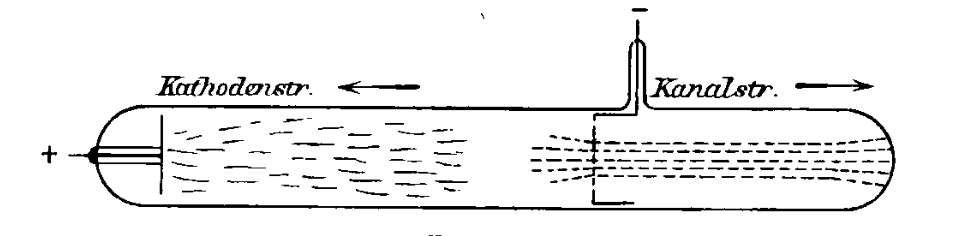
\includegraphics[scale=0.4]{StarkGas}
%DIFDELCMD <  %%%
\DIFdelendFL \DIFaddbeginFL 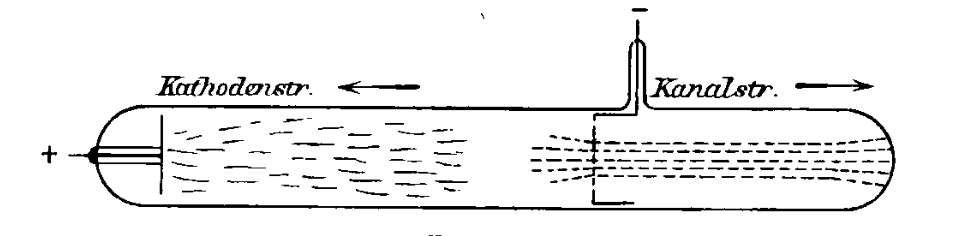
\includegraphics[scale=0.6]{StarkGas}
 \DIFaddendFL \caption{\label{fig:canal} Discharge tube producing cathode rays and canal rays \citep[405]{Stark1906}}
\end{figure}
%
Stark’s experimental investigations begin with a gas-filled discharge tube, typically containing hydrogen (\cref{fig:canal}). When an electrical discharge is applied, the discharge current is largely carried by fast negative electrons, which are accelerated by the electric field toward the anode. As these electrons traverse the gas, they undergo collisions with neutral atoms or molecules. In sufficiently energetic collisions, electrons are knocked out of atoms, producing positive ions, that is, \qt{atoms that have lost one or several negative electrons through ionization}{Atome, welche ein negatives Elektron oder mehrere Elektronen durch Ionisierung verloren haben} \citep[402]{Stark1906}. These ions are accelerated toward the cathode through a potential drop $V$ concentrated in the cathode fall, which sets the velocity scale of the moving ions. If the cathode is perforated, a fraction of the ions passes through the holes and continues beyond the cathode with approximately rectilinear motion, forming a beam propagating away from it. These beams of positive ions are known as canal rays \origg{Kanalstrahlen}, named after the \s{canals} in the cathode through which they pass \DIFdelbegin \DIFdel{\mbox{%DIFAUXCMD
\citep[403\todo{other pages}]{Stark1906}}\hskip0pt%DIFAUXCMD
}\DIFdelend \DIFaddbegin \DIFadd{\mbox{%DIFAUXCMD
\citep[403]{Stark1906}}\hskip0pt%DIFAUXCMD
}\DIFaddend .

When accelerated toward the cathode, the positive ions emit characteristic spectral radiation in all directions as a result of excitation processes in the discharge. Stark analyzed this radiation using a prism spectrograph. The emitted light entered the instrument through a narrow slit, which selected a well-defined direction of propagation (longitudinal or transverse with respect to the ion motion). After \DIFaddbegin \DIFadd{passing through }\DIFaddend the slit, the light is rendered approximately parallel and passed through a glass prism, which \DIFdelbegin \DIFdel{separates }\DIFdelend \DIFaddbegin \DIFadd{separated }\DIFaddend different wavelengths $\lambda$ by refraction; the dispersed radiation is finally recorded on a photographic plate. In the case of hydrogen, Stark took the Balmer series as empirically given, that is, as a set of well-defined spectral lines $\mathrm{H}\alpha$, $\mathrm{H}\gamma$, \dots \citep[417]{Stark1906}. Whether the emitting system consisted of neutral hydrogen in a discharge tube or of hydrogen ions in canal rays, the same characteristic lines reappeared. When the emitting ions moved along the line of sight of the spectrograph (toward $b$ or $c$ in \cref{fig:spectrograph}), Stark observed that the entire pattern of spectral lines was displaced toward longer wavelengths (redshift) for receding motion (toward $c$), and toward shorter wavelengths (blueshift) for approaching motion (toward $b$). The magnitude of this Doppler displacement increased with the ratio \betafactorh:
%
\begin{equation*}
\frac{\Delta\lambda}{\lambda} \sim \pm \frac{v}{c}.
\end{equation*}
%
Stark concluded that sharp line spectra \origg{Linienspektrum} are emitted by individual atomic ions in translational motion. By contrast, the \emph{band spectrum} \origg{Bandenspektrum}---consisting of groups of closely spaced lines forming characteristic bands---exhibited no measurable Doppler displacement. Stark therefore attributed band spectra to neutral atoms or molecular aggregates formed in recombination processes, whose translational velocities are much smaller than those of the canal-ray ions \citep[426]{Stark1906}.

In the first two parts of his paper, Stark established the ordinary first-order Doppler effect proportional to \betafactorh and concluded that \qt{\textins{t}he band spectrum and the line spectrum of hydrogen do not have the same carrier}{Das Bandenspektrum und das Linienspektrum des Wasserstoffs haben nicht denselben Träger} \citep[414]{Stark1906}. In part~III, he raised a further question: whether an additional displacement of spectral lines might exist that depends only on the magnitude of the ion’s velocity rather than on its direction. Any such effect would necessarily be proportional to \betafactorsquaredh, since linear terms change sign when the direction of motion is reversed, whereas quadratic terms do not \citep[409--10]{Stark1906}:
%
\begin{equation*}
\frac{\Delta\lambda}{\lambda} \sim \frac{1}{2}\frac{v^{2}}{c^{2}}.
\end{equation*}
%
To test for such a direction-independent effect, Stark arranged observations perpendicular to the direction of ion motion (the spectrograph $a$ in \cref{fig:spectrograph}). In this transverse configuration, the classical longitudinal Doppler effect vanishes by symmetry, since there is no velocity component along the line of sight.

Stark interpreted any residual shift as potentially dynamical in origin, arising from a velocity-dependent \qt{modification of the electromagnetic forces between the electrons, which is measured by even powers of the ratio $v/c$}{Modifikation der elektromagnetischen Kräfte zwischen den Elektronen, welche gemessen wird durch gerade Potenzen des Verhältnisses v/c} \citep[449]{Stark1906}. In Stark’s model, the ion as a \s{carrier} is not a rigid body but a physically deformable system, whose internal state can change with its motion and environment \citep[449]{Stark1906}. As the translational velocity of the ion increases, the amplitudes of the internal \s{centers} of emission (the electrons) were assumed to increase, since the strong electric fields required to accelerate the ions were thought to excite the bound electrons into oscillations of larger amplitude. Moreover, Stark speculated that radiation pressure acting on the oscillating electrons, the finite propagation speed of electromagnetic interactions, or deformation of the oscillatory system at high velocities might contribute to such effects. On this view, the combined action of increased electron amplitudes and radiation pressure could produce a physical deformation of the carrier, which Stark investigated as a possible mechanistic cause of wavelength shifts.

\begin{figure}
\centering
 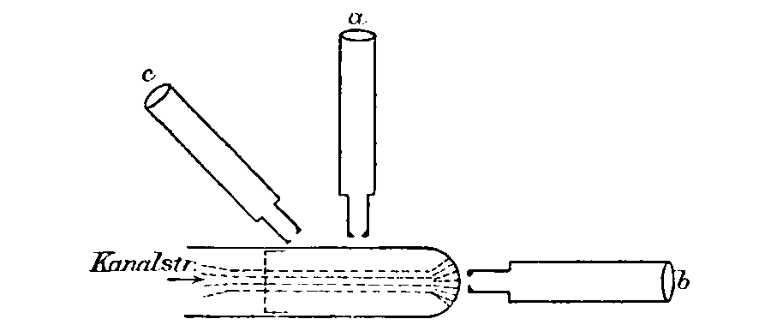
\includegraphics[scale=0.7, trim = 0mm 0mm 0mm 0mm, clip]{starkcanalspectrograph.png}
\caption{\label{fig:spectrograph} \DIFdelbeginFL \DIFdelFL{Set up }\DIFdelendFL \DIFaddbeginFL \DIFaddFL{Setup }\DIFaddendFL for observing the Doppler shift of canal-ray spectral lines, with spectrographs aligned parallel and perpendicular to the direction of propagation \citep[410]{Stark1906}}
\end{figure}
%
Stark reported tentative empirical indications consistent with this picture, noting a \DIFdelbegin \DIFdel{red shift }\DIFdelend \DIFaddbegin \DIFadd{redshift }\DIFaddend of the midpoints of certain spectral lines with increasing ion velocity—for example, a displacement of about $0.42\,\text{\AA}$ for the $\mathrm{H}\gamma$ line at a cathode fall of $7500$~Volts \citep[450]{Stark1906}. He emphasized, however, that while the attainable ion velocities were already sufficient to produce an observable longitudinal Doppler effect, which is first order in \betafactorh, they were still insufficient, in practice, for the transverse effect proportional to \betafactorsquaredh to be unambiguously isolated. In addition, he stressed the extreme experimental difficulty of ensuring exact transverseness. The slightest radial component would swamp the transverse effect. In particular, he calculated that a misalignment of only $1^\circ 59'$ would suffice to generate a spurious \DIFdelbegin \DIFdel{red shift }\DIFdelend \DIFaddbegin \DIFadd{redshift }\DIFaddend of comparable magnitude through the ordinary longitudinal Doppler effect. For these reasons, Stark explicitly characterized these observations as orienting indications rather than as conclusive experimental confirmation \citep[450--51]{Stark1906}.
\DIFdelbegin %DIFDELCMD < \todo{check}
%DIFDELCMD < %%%
\DIFdelend 

%What is relevant is that, in this context, Stark interpreted any putative second--order shift as a \emph{dynamical} effect, as defamation of the carrier of spectral line due its motion.

%He famously emphasized that relativity was not a complete theory; it merely imposed kinematical constraints on admissible theories. The new dynamics of the electron was obtained by modifying the classical dynamical laws governing charged point particles so as to bring them into conformity with the new kinematics. In this sense, relativity was not primarily a theory of the electron. Electrons in cathode and $\beta$-rays served chiefly to test the new point-particle dynamics, insofar as they could be treated as fast-moving charged particles \citep{Einstein1906c}. By contrast, developing a proper model of the electron conceived as a charge attached to a rigid body would have required a relativistic dynamics of rigid bodies, which had not yet been fully developed \citep{Einstein1907f}.




\DIFdelbegin %DIFDELCMD < \subsection{Einstein and Stark’s Second--Order Effect as a Test of Time Dilation}
%DIFDELCMD < %%%
\DIFdelend \DIFaddbegin \subsection{Einstein and Stark’s Second-Order Effect as a Test of Time Dilation}
\DIFaddend %
At that time, Einstein’s new dynamics of free electrons was under attack. The Einstein--Planck approach to electron dynamics was criticized by \citet{Ehrenfest1907}: since \DIFdelbegin \DIFdel{no\mbox{%DIFAUXCMD
\citep[197]{Einstein1907d}}\hskip0pt%DIFAUXCMD
n-spherical }\DIFdelend \DIFaddbegin \DIFadd{non-spherical }\DIFaddend electrons would, in principle, behave differently from spherical ones, the absence of a definite electron model was taken to be a defect rather than a virtue\DIFaddbegin \DIFadd{. }\DIFaddend \citet{Einstein1907a}, however, was not particularly impressed by this objection. He famously emphasized that relativity was not a complete theory, but merely imposed kinematical constraints on admissible theories. Einstein did not develop a theory of the electron, but modified the equations of motion of a charged particle in general so as to make them Lorentz invariant. After coming across \citets{Stark1906} paper toward the end of 1906, Einstein may have quickly realized that this work opened the possibility of a more direct test of the new kinematics itself, without recourse to electron dynamics. He addressed this issue in a paper submitted on \datemy{3}{3}{1907}.

Stark’s experiments showed that wave sources moving at very high velocities were in fact available: the positive ions forming canal rays emit line spectra that exhibit a longitudinal \DIFdelbegin \DIFdel{first--order }\DIFdelend \DIFaddbegin \DIFadd{first-order }\DIFaddend Doppler effect, that is, an effect proportional to \betafactorh due to their motion. As we have seen, Stark also attempted to detect an additional \DIFdelbegin \DIFdel{second--order }\DIFdelend \DIFaddbegin \DIFadd{second-order }\DIFaddend effect, proportional to \betafactorsquaredh; however, the experimental setup, not specifically designed for this purpose, was insufficient to yield a reliable result. Nevertheless, it was shown that, in principle, it was possible to decide whether the spectral lines of \DIFdelbegin \DIFdel{fast--moving }\DIFdelend \DIFaddbegin \DIFadd{fast-moving }\DIFaddend ions exhibit a redshift when they are observed spectroscopically at right angles to the direction of motion. Einstein’s aim was to show that the principle of relativity, together with the principle of the constancy of the velocity of light, suffices to account for the effect in question \citep[197]{Einstein1907d}. It is worth noting, however, that Einstein did not present Stark’s work as a test of the relativistic wave equation as a whole, but rather as a test specifically of time dilation, since in the transverse case the effect depends solely on the time transformation.

%In a paper submitted on \datemy{3}{3}{1907}, \citet{Einstein1907d}   occurs  of the ions.  

Referring to his earlier 1905 paper, Einstein reminds his readers that\DIFaddbegin \DIFadd{, }\DIFaddend in relativity theory\DIFaddbegin \DIFadd{, }\DIFaddend a uniformly moving clock runs more slowly, when judged from a \s{stationary} system\DIFdelbegin \DIFdel{, than when judged }\DIFdelend \DIFaddbegin \DIFadd{: successive ticks of a clock at rest in $K'$ are assigned a longer coordinate-time interval by the synchronized clocks at rest in a }\s{stationary} \DIFadd{system $K$ than }\DIFaddend by an observer co-moving with the clock. Einstein appears implicitly to assume that any periodic system passing through identical phases can be regarded as a clock. If $\nu_0$ denotes the frequency defined as the number of periods $N$ divided by the time interval $\Delta t'$ measured in the co-moving system $K'$, and $\nu$ denotes the frequency defined as the same number $N$ divided by the coordinate time interval $\Delta t$ measured in a system $K$ relative to which the atom is moving, then, since $\Delta t=\gamma\,\Delta t'$, special relativity predicts:


%The spectral lines of ions are nothing but a physical realization of clocks moving at hight velocity. The connection between the \tDe and time dilation becomes rather transparent once one recalls that color corresponds to the wavelength $\lambda$ or, equivalently, to the frequency $\nu$ of light, that is, to the number of wave crests received per \emph{unit time} as measured by a clock, the two being related in vacuum by the wave relation $c = \lambda \nu$. Since the wave propagates at the fixed speed $c$, any change in the temporal period of the oscillation is necessarily mirrored in a change in the spatial separation of successive wavefronts. In this sense, the atomic ions of the canal rays, which emit and absorb radiation of definite frequencies, may be regarded as rapidly moving clocks.

%If the frequency $\nu$ denotes the number oscillation of the ion per unit time $t$ as measured by the stationary observer, and $\nu_0$ the corresponding number measured by the co-moving observer, then

%\begin{equation*}
%\frac{\nu}{\nu_0}
%= \frac{\displaystyle \frac{N}{\Delta t}}{\displaystyle \frac{N}{\Delta t'}}
%= \frac{\Delta t'}{\Delta t}
%= \sqrt{1-\betafactorsquared},
%\end{equation*}


\begin{equation}\label{eq:doppler}
\frac{\nu}{\nu_0}=\sqrt{1-\betafactorsquared},
\end{equation}
%
Testing this relation requires clocks that can be accelerated to very high velocities without compromising their accuracy. Direct experimental verification using mechanical clocks is therefore likely to remain unattainable, since the velocities that can be imparted to such devices are negligible in comparison with the speed of light. Nature, however, provides systems that effectively function as clocks and that can be accelerated, by means of an electric field, to extremely high speeds: \qt{The atom ion of the canal rays, which emits and absorbs radiation of definite frequencies, is therefore to be regarded as a rapidly moving clock, and the relation just given is thus applicable to it}{Das Strahlung von bestimmten Frequenzen aussendende und absorbierende Atomion der Kanalstrahlen ist nun als eine rasch bewegte Uhr aufzufassen, und es ist daher die soeben angegebene Beziehung auf dasselbe anwendbar} \citep[198]{Einstein1907d}.

One might object that the frequency $\nu_0$ of the fast-moving ion cannot be measured by a co-moving spectrograph. However, according to Einstein, there was sufficient evidence to support the claim that, whether the emitting system consisted of neutral hydrogen in a discharge tube or of hydrogen ions produced in canal rays, the same characteristic spectral lines reappeared. This was taken as strong evidence that the Balmer series expresses a stable property of the hydrogen system, rather than something contingent on the manner in which it was produced. Einstein could then point out that the corresponding frequencies are determined solely by the nature of the ion—that is, ions of the same species yield the same frequency $\nu_0$ when measured with a spectrograph at relative rest:

\qt{However, one has to take into consideration that the frequency $\nu_0$ (for the co-moving observer) is unknown, so that the above relation is not accessible to direct experimental verification. But, it may be assumed that $\nu_0$ is also equal to the frequency emitted or absorbed by the same ion while at rest, and this for the following reason. From the fact that one and the same line spectrum is formed under very different conditions, we conclude that the frequency $\nu_0$ does not depend on interactions between moving ions and the stationary gas, but is a characteristic of the ion only; from this one directly concludes with the help of the principle of relativity that $\nu_0$ must equal the frequency of radiation emitted or absorbed by an ion at rest}{Es ist aber zu beachten, da $\beta$ die Frequenz $\boldsymbol{v}_0$ (für den mitbewegten Beobachter) unbekannt ist, so daß die obige Beziehung der experimentellen Prüfung nicht direkt zugänglich ist. Es ist aber anzunehmen, daß $v_0$ auch gleich ist der Frequenz, welche dasselbe Ion im ruhenden Zustand emittiert bez. absorbiert, und zwar aus folgendem Grunde. Aus der Tatsache, daß dasselbe Linienspektrum unter sehr verschiedenen Bedingungen entsteht, entnehmen wir, daß die Frequenz $v_0$ nicht abhängig ist von Wechselwirkungen zwischen bewegten Ionen und ruhendem Gas, sondern daß sie dem Ion allein eigentümlich ist; hieraus folgert man direkt mit Hilfe des Relativitätsprinzips, daß $\boldsymbol{v}_0$ gleich sein muß der Frequenz der von einem ruhenden Ion emittierten bez. absorbierten Strahlung.}[\citep[198]{Einstein1907d}]
%
Einstein then assumes that ions of a given species can be treated as identical systems: the recurrence of the same sharp spectral lines under widely varying experimental conditions supports the assumption that their characteristic frequencies $\nu_0$ are intrinsic properties of the ions themselves and do not depend on interactions with the surrounding medium. That is, all ions of the same species exhibit the same spectral lines when at relative rest. Since canal-ray ions move at very high velocities, any possible shift $\nu$ of the spectral lines with respect to $\nu_0$ would thus become, at least in principle, empirically accessible.

%Einstein could not test this assumption in the sense that one cannot place a spectrograph co-moving with fast moving ions. However, spectrographic evidence in favor of this assumption was strong. 



The \DIFdelbegin \DIFdel{first--order }\DIFdelend \DIFaddbegin \DIFadd{first-order }\DIFaddend Doppler effect arises from the relative motion between source and observer and depends linearly on \betafactorh. In classical theory it does not presuppose any particular microphysical account of the emission process, nor does it require modifications of the internal dynamics of the emitter. In Stark’s work, however, the \DIFdelbegin \DIFdel{second--order }\DIFdelend \DIFaddbegin \DIFadd{second-order }\DIFaddend Doppler effect—that is, any frequency shift proportional to \betafactorsquaredh observed in a transverse configuration—could not be explained by simple relative motion along the line of sight. Stark therefore treated the effect as a genuinely dynamical modification of the \s{carrier}: he assumed that uniform motion produces a real change in the emission process of fast ions---a kind of reduction in the number $N$ of oscillations completed \DIFdelbegin \DIFdel{during a }\emph{\DIFdel{same time}} %DIFAUXCMD
\DIFdelend \DIFaddbegin \DIFadd{by the moving ion during the same universal time }\DIFaddend interval (frequency contraction). Einstein explicitly rejected this dynamical explanation. Instead, he invoked the principle of relativity to support the assumption that uniform motion does \emph{not} alter the internal oscillatory processes of the ion\DIFdelbegin \DIFdel{; the number }\DIFdelend \DIFaddbegin \DIFadd{. The same emission process involves the same count }\DIFaddend $N$ of \DIFdelbegin \DIFdel{oscillations associated with a given emission process is the same in all non-accelerated systems, but spread over }\emph{\DIFdel{different}} %DIFAUXCMD
\DIFdel{time intervals time dilation)}\DIFdelend \DIFaddbegin \DIFadd{completed oscillations; the relativistic effect arises because this same count is referred to different time intervals in the two inertial descriptions}\DIFaddend .

%DIF > \(N_{\mathrm{mov}}<N_{\mathrm{rest}}\) 
\DIFaddbegin 

\DIFaddend This assumption is the key to Einstein’s reasoning. The \DIFdelbegin \DIFdel{number $N$ of oscillations is }\DIFdelend \DIFaddbegin \DIFadd{intrinsic frequency $\nu_0=N/\Delta t'$ is taken to be }\DIFaddend fixed, and longitudinal Doppler components are excluded by definition. As a consequence, the remaining transverse Doppler effect, that is, the reduced observed frequency $\nu = N/\Delta t = \nu_0/\gamma$, can \emph{only} be attributed to the transformation properties of the time coordinate between inertial reference systems in uniform relative motion, $\Delta t=\gamma\Delta t'$, as prescribed by Einstein’s new kinematics. The \tDe thus serves as a test of the \DIFdelbegin \DIFdel{time--dilation }\DIFdelend \DIFaddbegin \DIFadd{time-dilation }\DIFaddend relation. Expanding \cref{eq:doppler} in a series, \citet[197]{Einstein1907d} obtains, to second order in \betafactorh,
%
\begin{equation}\label{eq:cumulativedoppler}
\frac{\nu-\nu'}{\nu'} \approx -\frac{1}{2}\left(\frac{v}{c}\right)^2\,,
\end{equation}
%
which quantifies this deficit. Equation~\eqref{eq:cumulativedoppler} therefore provides a direct theoretical expression for the sought \DIFdelbegin \DIFdel{second--order }\DIFdelend \DIFaddbegin \DIFadd{second-order }\DIFaddend effect in the radiation emitted by fast \DIFdelbegin \DIFdel{canal--ray }\DIFdelend \DIFaddbegin \DIFadd{canal-ray }\DIFaddend ions.

Equation~\eqref{eq:cumulativedoppler} can be tested experimentally by means of a spectrograph oriented such that the motion of the emitting ions is perpendicular to the line of sight; in this configuration, all \DIFdelbegin \DIFdel{first--order }\DIFdelend \DIFaddbegin \DIFadd{first-order }\DIFaddend Doppler contributions vanish. A spectrograph registers the wavelength at which a given spectral line appears after dispersion. The observed position of a spectral line therefore determines its wavelength $\lambda$, and, via the relation $\lambda = c/\nu$, its frequency $\nu$. By comparing the wavelength $\lambda$ of the line emitted by the moving ions with the reference wavelength $\lambda_0$ measured for ions at rest, the spectrograph allows one to determine the fractional shift $(\lambda-\lambda_0)/\lambda_0$, which is equivalent (up to a change of sign) to $(\nu-\nu_0)/\nu_0$. Comparing the relativistic prediction with Stark’s experimental results, Einstein noted that the numerical values reported by Stark exceeded the expected effect by more than an order of magnitude. However, he expressed skepticism regarding the reliability of the existing measurements \citep[198]{Einstein1907d}. Nevertheless, in correspondence with Stark in April~1907, Einstein expressed the hope that it might eventually become possible to detect such \DIFdelbegin \DIFdel{second--order }\DIFdelend \DIFaddbegin \DIFadd{second-order }\DIFaddend effects experimentally with greater accuracy \lettercpaep{Einstein}{Stark}{13}{4}{1907}[5][45].

\DIFaddbegin \medskip
\DIFaddend %Under the assumption that the number of oscillations $N$ associated with the emission process is fixed, one might claim that what is effectively tested is the excess of the elapsed time assigned to the same process in the non--co--moving frame $K$ with respect to $K'$, that is,
%%
%\begin{equation*}
%\frac{\Delta t-\Delta t'}{\Delta t'}
%\approx
%\frac{1}{2}\left(\frac{v}{c}\right)^{2}.
%\end{equation*}
%%

%Consider a fixed emission process that produces a definite number of light pulses, say $N$. That number is fixed by the physical process itself and is the same for all observers. What differs between observers is how densely those same pulses are distributed along their time axis. For an observer co–moving with the source, the $N$ pulses are emitted and received over a time interval $\Delta t’$. For an observer relative to whom the source is moving, the very same $N$ pulses are spread over a longer time interval $\Delta t=\gamma\Delta t’$. In this precise sense, the pulses are less densely packed along the time axis of the non–co–moving system.


\subsection{The \TDE{} in Einstein’s 1907/1908 \german{Jahrbuch} Paper}
%
Stark was the editor of the \emph{Jahrbuch der Radioaktivität und Elektronik}. In September, he invited Einstein to contribute a comprehensive review article on the theory of relativity, \DIFaddbegin \DIFadd{and }\DIFaddend Einstein agreed to \q{deliver the desired report} \lettercpaep{Einstein}{Stark}{25}{9}{1907}[5][58]. Stark assisted him by supplying relevant literature that the young Einstein could not easily access \lettercpaep{Einstein}{Stark}{7}{10}{1907}[5][61]. The paper was ultimately submitted on \datef{4}{12}{1907} and appeared in the \DIFdelbegin %DIFDELCMD < \jt{Jarbuch} %%%
\DIFdelend \DIFaddbegin \jt{Jahrbuch} \DIFaddend at the end of \DIFdelbegin %DIFDELCMD < \datef{22}{1}{1908}%%%
\DIFdel{. }\DIFdelend \DIFaddbegin \DIFadd{January~1908. }\DIFaddend Beyond synthesizing his earlier relativity work, \DIFdelbegin \DIFdel{the }\DIFdelend \citet{Einstein1908} incorporated several recent developments, including \citets{Laue1907} derivation of the drag coefficient, \citets{Planck1906a} reformulation of relativistic dynamics, and related advances in the treatment of thermodynamics within the relativistic framework \citep{Planck1907}. As expected, Einstein also used the 1908 review to discuss \citets{Stark1906} observations as a possible means of testing the new kinematics.

A distinctive feature of Einstein’s new presentation is that the transverse Doppler effect is no longer treated primarily as a consequence of the Lorentz-invariant wave equation, but is instead relocated within the kinematical framework of the theory. Stark’s work on the second-order transverse Doppler effect is mentioned explicitly in the kinematical part \rom{1} of Einstein’s paper, where time dilation is discussed as one of the consequences of the new kinematics \citep[422]{Einstein1908}. In the electrodynamic part \rom{2}, by contrast, Einstein derives the Lorentz-invariant wave equation and hence the relativistic Doppler effect without explicitly distinguishing between longitudinal and transverse cases. Although Stark is not mentioned in this context, Einstein does point out that the relativistic Doppler effect can be tested by measuring the frequency shift of light emitted or absorbed by canal rays, which depends both on the velocity of the ions and on the direction in which the radiation is observed \citep[425]{Einstein1907a}. At the time, canal rays were essentially the only laboratory sources capable of reaching velocities sufficiently large for such effects to be spectroscopically accessible.

%To simplify the presentation, one can start with two non-accelerated coordinate systems, $K$ and $K'$, whose origins and standard clocks $U$ and $U'$ coincide at an initial instant. The clocks are identical, that is, they tick at the same rate $\nu_0$, and are synchronized at the same place and time using light rays; in other words, they tick in phase. The system $K'$ moves uniformly with velocity $v$ relative to $K$. The clock $U'$ is assumed to be permanently at rest at the origin of the moving system $K'$.


%2. At the origin of coordinates of $S'$ there is placed a clock at rest, which runs $v_0$ times faster than the clocks used for time measurement in the systems $S$ and $S'$, that is, this clock executes $2o$ periods in a time interval during which the reading of a clock at rest relative to it, of the kind used for time measurement in $S$ and $S'$, increases by one unit.

In this way, the discussion of the transverse Doppler effect is conceptually shifted from the domain of optics and electrodynamics to that of kinematics \DIFdelbegin \DIFdel{\mbox{%DIFAUXCMD
\citep[421-22]{Einstein1908}}\hskip0pt%DIFAUXCMD
}\DIFdelend \DIFaddbegin \DIFadd{\mbox{%DIFAUXCMD
\citep[421--22]{Einstein1908}}\hskip0pt%DIFAUXCMD
}\DIFaddend . The presentation of the time-dilation effect here differs significantly from that of the 1905 paper: it places far less emphasis on algebraic derivation and is instead oriented toward clarifying the physical interpretation and the prospective experimental testability of the effect. Einstein \DIFdelbegin \DIFdel{considers again }\DIFdelend \DIFaddbegin \DIFadd{again considers }\DIFaddend a clock $U'$ permanently at rest at $x'=0$, at the origin of the moving system $K'$, which moves uniformly with velocity $v$ relative to $K$ along the $x$-axis. The clock is modeled as a physical periodic system with an intrinsic rest frequency $\nu_0$. The intrinsic frequency $\nu_0$ characterizes the clock as a physical system and is assumed to be independent of its state of uniform motion. Accordingly, the successive ticks of the clock \DIFdelbegin \DIFdel{are invariantly }\DIFdelend \DIFaddbegin \DIFadd{can be }\DIFaddend labeled by the integers $n=1,2,3,\ldots$, corresponding to the completion of successive periods of the same physical process.
\DIFdelbegin \DIFdel{In this sense, the number $N$ of ticks associated with a given physical process used as a clock is assumed from the outset to be invariant.
}\DIFdelend 

Since the clock $U'$ is at rest in $K'$, that is, since $\Delta x'=0$, its successive ticks occur at equal intervals of the time coordinate $t'$:
%
\begin{equation*}
t_n'=\frac{n}{\nu_0},
\end{equation*}
%
where the relation between the discrete tick number $n$ and the continuous time coordinate $t'$ is fixed by the convention that assigns the rate $\nu_0$ to the clock. Accordingly\footnote{In the following I also rely on \DIFdelbegin \DIFdel{\mbox{%DIFAUXCMD
\citep[131-32]{Einstein1910} }\hskip0pt%DIFAUXCMD
}\DIFdelend \DIFaddbegin \DIFadd{\mbox{%DIFAUXCMD
\citealp[131--32]{Einstein1910} }\hskip0pt%DIFAUXCMD
}\DIFaddend to clarify Einstein’s otherwise somewhat elliptical reasoning}, the time instants at which successive periods are completed in the system $K'$ are
%
\begin{equation*}
t_1'=\frac{1}{\nu_0}, \quad
t_2'=\frac{2}{\nu_0}, \quad
t_3'=\frac{3}{\nu_0}, \quad \cdots \quad
t_n'=\frac{n}{\nu_0}.
\end{equation*}
%
Einstein then asks how fast this same clock runs when viewed from the system $K$. To answer this question, he determines the coordinate times in $K$ at which the successive periods of the moving clock are completed. These times are obtained by applying the Lorentz transformation to the time coordinate of $K'$:
%
\begin{equation*}
t=\gamma \left(t^{\prime}-\frac{v}{c^2} x^{\prime}\right).
\end{equation*}
%
Since the clock $U'$ remains permanently at rest at the origin of $K'$, one always has $x^{\prime}=0$. The coordinate time in $K$ corresponding to the completion of the $n$th period is therefore
%
\begin{equation*}
t_n=\gamma t_n'=\frac{\gamma}{\nu_0}\,n.
\end{equation*}
%
Accordingly, the successive periods of the moving clock $U'$ are completed, in the system $K$, at the time instants
%
\begin{equation*}
t_1=\gamma\,\frac{1}{\nu_0}, \quad
t_2=\gamma\,\frac{2}{\nu_0}, \quad
t_3=\gamma\,\frac{3}{\nu_0}, \quad \cdots \quad
t_n=\gamma\,\frac{n}{\nu_0}.
\end{equation*}
%
Comparing the coordinate-time differences $t_n-t_1$ and $t_n'-t_1'$ assigned to the same \DIFdelbegin \DIFdel{1rs }\DIFdelend \DIFaddbegin \DIFadd{first }\DIFaddend and $n$th tick of $U'$ in the two systems $K$ and $K'$, one finds that
%
\begin{equation*}
\Delta t=\gamma\,\Delta t'.
\end{equation*}
%
The frequency of the clock $U'$ at rest in $K'$ is $\nu_0$. When the same clock is described from the system $K$, the same number $N$ of periods is distributed over a longer elapsed coordinate-time interval $\Delta t=\gamma\,\Delta t'$. From the standpoint of $K$, $U'$ \DIFdelbegin \DIFdel{appears therefore to have }\DIFdelend \DIFaddbegin \DIFadd{therefore appears to have a }\DIFaddend reduced frequency $\nu$:
%
\begin{equation}\label{eq:frequency}
\nu = \frac{N}{\Delta t} = \frac{N}{\gamma\,\Delta t'} = \nu_0 \sqrt{1-\frac{v^2}{c^2}}.
\end{equation}
%
In this precise sense, \DIFaddbegin \DIFadd{one can say that }\DIFaddend the moving clock runs \s{more slowly} than an identical clock at rest in $K$\DIFaddbegin \DIFadd{: the ticks of the moving clock are assigned a longer coordinate-time interval by the synchronized clocks at rest in $K$ than the ticks of an identical clock at rest in $K$}\DIFaddend .

\DIFdelbegin \DIFdel{This statement}\DIFdelend \DIFaddbegin \DIFadd{The claim that the moving clock runs }\s{more slowly}\DIFaddend , however, must be treated with some caution. As one can see, Einstein’s argument rests on the fundamental assumption that clocks are \emph{physically identical} across \DIFdelbegin \DIFdel{non--accelerated }\DIFdelend \DIFaddbegin \DIFadd{non-accelerated }\DIFaddend reference frames, that is, that they possess the same intrinsic frequency \DIFdelbegin \DIFdel{$\nu_0$ }\DIFdelend \DIFaddbegin \DIFadd{$\nu_0=N/\Delta t'$ }\DIFaddend independently of their uniform motion. Under this assumption, \DIFdelbegin \DIFdel{the number $N$ of periods is taken to be invariant, and }\DIFdelend time dilation is attributed \DIFdelbegin \DIFdel{entirely to the expansion of the elapsed }\DIFdelend \DIFaddbegin \DIFadd{to the dilation of the }\DIFaddend coordinate-time interval $\Delta t$ \DIFaddbegin \DIFadd{assigned in $K$ to the same number $N$ of completed periods of the moving clock}\DIFaddend . One of the most significant novelties of Einstein’s 1908 paper is that he made this assumption explicit for the first time: \qt{the rate of a clock does not undergo any permanent change if such objects are set in motion and then brought to rest again}{Ganggeschwindigkeit einer Uhr dadurch keine dauernde Änderung erleiden, daß diese Gegenstände in Bewegung gesetzt und wieder zur Ruhe gebracht werden} \citep[420\fn{1}]{Einstein1908}. If the clock $U'$ were carefully brought to rest and placed next to any of the clocks $U$ at rest in $K$, the two would run at the same rate $\nu_0$. This requirement may therefore be taken as a criterion for a \s{good} clock, namely one whose rate is not permanently affected by its past history%
%
\footnoteh{As Einstein had pointed out in his first 1905 paper (but not in the 1907/1908 paper), initially synchronized identical \s{ideal} clocks that move along closed polygonal paths and subsequently meet again are expected to tick at the same rate (that is, there is no second-clock effect), though they will no longer be synchronized. The clock transported along a non-inertial path will lag behind an identical clock left at rest by an amount proportional to $t(v^{2}/c^{2})$, where $t$ is the travel time. Despite the frame-dependent character of time dilation, the resulting non-synchronicity in their indications is ineliminable, cannot be removed by a mere change of coordinates, and must be treated as an objective fact}.

To test the relation \cref{eq:frequency} empirically, one requires the existence of a physical system that actually behaves in this way, that is, a real clock capable of reproducing the same time units in different \DIFdelbegin \DIFdel{non--accelerated }\DIFdelend \DIFaddbegin \DIFadd{non-accelerated }\DIFaddend reference frames. \emph{If} such a system exists, \emph{then} the consequences of the new kinematics for time become empirically accessible. As we have seen, nature offers objects that possess the character of ideal clocks, namely ions emitting spectral lines:
%
\qt{The formula $\nu=\nu_0 \sqrt{1-\frac{v^2}{c^2}}$ admits of a very interesting application. Mr. J. Stark showed in the previous year that the ions forming canal rays emit line spectra, by observing a displacement of spectral lines that is to be interpreted as a Doppler effect. Since the oscillation process that corresponds to a spectral line is to be considered an intra-atomic process \textit{whose frequency is determined by the ion alone}, we may consider such an ion as a clock of a certain frequency $\nu_0$, which can be determined, for example, by investigating the light emitted by \myemph{identically constituted} ions which are at rest relative to the observer. The above consideration shows, then, that the effect of motion on the light frequency that is to be ascertained by the observer is not completely given by the \textins{longitudinal} Doppler effect. The motion also reduces the (\myemph{apparent}) proper frequency of the emitting ions in accordance with the relation given above}{Da der einer Spektrallinie entsprechende Schwingungsvorgang wohl als ein intraatomischer Vorgang zu betrachten ist, dessen Frequenz durch das Ion allein bestimmt ist, so konnen wir ein solches Ion als eine Uhr von bestimmter Frequenzzahl $\nu_o$ ansehen, welch letztere man z. B. erhālt, wenn man das von gleich beschaffenen, relativ zum Beobachter ruhenden Ionen ausgesandte Licht untersucht. Die obige Betrachtung zeigt nun, daß der Einfluß der Bewegung auf die von dem Beobachter zu ermittelnde Lichtfrequenz durch den Dopplereffekt noch nicht vollstāndig gegeben ist. Die Bewegung verringert vielmehr außerdem die (scheinbare) Eigenfrequenz der emittierenden Ionen gemäß obiger Beziehung}[\citep[422\me]{Einstein1908}]
%
This passage makes clear that the premise of the argument is that ions of the same species are taken to be physically identical when compared at relative rest; they are all \s{identically constituted}. By 1908, spectroscopy had established with great precision that atoms and ions of the same species emit sharp, reproducible spectral lines whose frequencies are invariant across laboratories and experimental conditions, provided the emitters are compared at rest. This empirical stability strongly suggested that atomic emission frequencies $\nu_0$ are intrinsic properties of the emitters, not contingent on macroscopic conditions or preparation histories. Despite the lack of a theoretical explanation, for Einstein this made the atom, the \qt{producer of spectral lines}{Erzeuger der Spektrallinien} \citep[459]{Einstein1908}, uniquely well suited to function as a natural clock.

Since ions are assumed to be identical in all frames in uniform relative motion, the frequency shift of fast-moving ions measured by a spectrograph at rest cannot be attributed to a change in the ions themselves. In the longitudinal case, the observed shift may still be explained by motion along the line of sight. By contrast, for a spectrograph oriented perpendicular to the direction of motion, no such explanation is available. In this case, the observed redshift must be understood as a consequence of time dilation alone. For this reason, Einstein described the redshift as \emph{apparent}\footnote{If a transversely moving source produces a redshift $\nu=\gamma^{-1}\nu_0$, then a transversely moving spectrograph relative to a source at rest produces the inverse effect, a blueshift $\nu=\gamma\nu_0$. The two situations are completely symmetrical in principle, but only the redshift from a transversely moving source is usually referred to as the transverse Doppler effect. While fast-moving atoms are readily available in canal rays, fast-moving spectrographs are not experimentally feasible. Nevertheless, this symmetry shows that the transverse Doppler effect cannot be attributed to a real, direction-dependent dynamical deformation of the atom}. The reduction in frequency is frame dependent and \DIFdelbegin \DIFdel{disappears entirely for }\DIFdelend \DIFaddbegin \DIFadd{is not recorded by }\DIFaddend a spectrograph co-moving with the ion. The adjective \emph{apparent} was likely chosen to contrast the relativistic account with Stark’s dynamical interpretation.

As we have seen in \cref{sub:stark}, in Stark’s view, the motion of the ion produces a \emph{real} frequency contraction, that is, a modification of the emitting system’s intrinsic oscillation frequency $\nu_0$, such that \DIFdelbegin \DIFdel{the ion completes a smaller number $N$ of oscillations in the }\emph{\DIFdel{same}} %DIFAUXCMD
\DIFdel{time interval $\Delta t'$ }\DIFdelend \DIFaddbegin \DIFadd{fewer oscillations are completed during a given time interval }\DIFaddend in the moving frame. In Einstein’s kinematical interpretation, by contrast, the intrinsic periodic process remains unchanged, since it is fixed by the same physical emission mechanism. The \DIFdelbegin \DIFdel{number $N$ of oscillations associated with a given emission process is invariant. The }\DIFdelend observed redshift is therefore not due to a change in the emitter’s frequency $\nu_0$, but to time dilation: relative to a frame $K$ in which the ion is moving\DIFdelbegin \DIFdel{the same number of oscillations $N$ is }\DIFdelend \DIFaddbegin \DIFadd{, the same completed oscillations are }\DIFaddend distributed over a \emph{longer} time interval $\Delta t=\gamma\Delta t'$ than in the rest frame $K'$. The frequency shift is thus explained by the relativistic transformation of the time coordinate, not by a dynamical modification of the source. However, Einstein clearly regarded this \s{apparent} effect as an unavoidable consequence of the theory and as one that could, in principle, be empirically detected. 

Since the effect is of second order in $\betafactorh$, it requires clocks moving at sufficiently high velocities, a condition satisfied by ions in canal rays. If two identical spectrographs are at rest with respect to the source but operate for different exposure times, the longer exposure merely collects a larger number $N$ of wave crests: both the elapsed time and the number of accumulated oscillations increase proportionally. As a result, the inferred frequency $\nu_0$ remains unchanged, and the spectral lines appear at the same position; only the intensity varies. In the relativistic case, by contrast, the crucial point is that the same physical emission process is described from two different non-accelerated frames. The same number of oscillations $N$ associated with a given emission process is thus referred to different elapsed times, $\Delta t=\gamma \Delta t'$. The difference in the temporal interval over which the same oscillations $N$ are distributed necessarily entails a change in the observed frequency $\nu$. Through the relation $\lambda = c/\nu$, this difference in temporal rate is translated into a difference in wavelength, which the spectrograph at rest in $K$ registers directly as a redshift of the atom’s spectral line.


\section{Ritz and the Transverse Doppler Effect as an \emph{Experimentum Crucis}}
%
Replying to a letter from Sommerfeld that is no longer extant, Einstein expresses strong interest in having a \DIFdelbegin \DIFdel{canal--ray }\DIFdelend \DIFaddbegin \DIFadd{canal-ray }\DIFaddend experiment carried out and welcomes Sommerfeld’s willingness to involve Peter Paul Koch (at that time an assistant of Wilhelm Röntgen in Munich) in testing the \tDe. Einstein nevertheless betrays some caution as to whether Koch would actually carry out the experiments \lettercpaep{Einstein}{Sommerfeld}{14}{1}{1908}[5][73]. He notes that Stark had already informed him some months earlier of his intention to undertake the same investigation, although Stark had since written to Einstein repeatedly without again mentioning the experiment \lettercpaep{Einstein}{Sommerfeld}{14}{1}{1908}[5][73]. The letter to Sommerfeld also shows that this was something of a side issue. The main point of debate concerned the empirical test of the variability of the electron mass investigated by Kaufmann. Indeed, Einstein’s 1908 paper devotes the entire \S10 to a discussion of Kaufmann’s experiments and to a comparison between the different predictions of the Abraham electron, the Einstein--Lorentz electron, and the Bucherer electron \citep{Walter2018}.

%Kaufmann’s results did not confirm relativity. Einstein did not seem particularly worried, given that the experimental techniques then available were unlikely to deliver accurate quantitative confirmations.
%
\footnoteh{This discussion is framed against the background of the fact that Kaufmann’s results did not confirm relativity. Einstein did not seem particularly worried, given that the experimental techniques then available were unlikely to deliver accurate quantitative confirmations. The theory yielded a tightly interconnected series of consequences, all of which stood or fell together, as Einstein put it, \q{theoretical systems which embrace a larger complex of phenomena} \citep{Einstein1907a}. The appeal of the theory lay in its logical rigidity: it was highly implausible that a single phenomenon should diverge while the rest of the system held together. Once it successfully accounted for phenomena such as aberration, the Fizeau experiment, and the Michelson experiment\etc, a qualitative convergence of Kaufmann-like experiments sufficed to support it. For this reason, isolated experimental \emph{quantitative} anomalies did not immediately threaten his confidence in the theory, since they appeared to move \emph{qualitatively} in the right direction \citep{Hentschel1992a}. This attitude must also have shaped Einstein’s response to the lack of confirmation of the \tDe}


%\footnote{see, \cite{Martinez2004-04}. Regarded at the time as a \s{rising star} of European physics, Ritz was, like Einstein, trained at the Zurich Polytechnic from 1897 to 1901 and later became closely acquainted with electron theory during his time in Göttingen. Although he is today best known in atomic physics (the Rayleigh-Ritz perturbation theory and the Ritz combination principle), Ritz became increasingly skeptical of Lorentz-Maxwell electrodynamics after his stay Leiden with in summer of 1903 his close friend \Ehr where he could follow Lorentz lectures}

%\subsection{Ritz and the \TDE}
%
These electron models were all constructed within a theoretical context shaped by the assumed validity of Maxwellian electrodynamics and by constraints imposed by optical and electrodynamic phenomena, even though they differed markedly in their interpretations of the status and significance of the Lorentz transformations. A more radical challenge to relativistic kinematics was posed by Ritz, who in the winter of 1907--1908 moved from Göttingen to Tübingen, where he worked with the experimentalist Friedrich Paschen. Regarded as a rising star of European physics for his work in spectral theory \citep{Hentschel2012}, Ritz became increasingly skeptical of Lorentz--Maxwell electrodynamics after a stay in Leiden with his close friend \Ehr \citep{Martinez2004-04}. His major polemical paper appeared in the \emph{Annales de chimie et de physique} in February 1908, only a few weeks after the publication of Einstein’s 1908 review article. Like Einstein, \citet[147--48]{Ritz1908a} was skeptical of the reliability of Kaufmann’s experiments. However, for him, the difficulties involved in constructing a suitable model of the electron and in accounting for the velocity dependence of its mass were not isolated technical problems but rather symptoms of a deeper flaw in Maxwell--Lorentz electrodynamics itself.

% For Ritz, these difficulties were not isolated technical problems but symptoms of a deeper flaw in Maxwell-Lorentz’s electrodynamics itself. Ritz argued that Kaufmann’s experiments on the electric and magnetic deflection of radium \(\beta\)-rays do not demonstrate that the electron’s mass is entirely of electromagnetic origin or that it depends on its absolute velocity. Such a conclusion, he maintained, presupposes the validity of the Lorentz force law at high velocities, an assumption not compelled by experiment. By contrast, the apparent increase in the electron’s mass could instead be attributed to a reduction in the electromagnetic force acting on rapidly moving electrons relative to the value predicted by the Lorentz force law. Ritz also questioned the stability of such electron models, maintaining that an extended charged body governed solely by electromagnetic self-forces could not be shown to possess a stable equilibrium without introducing additional, non-electromagnetic assumptions.

Lorentz--Maxwell electrodynamics assumes the existence of an absolute system of ether coordinates, taken to be independent of the motions of matter, with respect to which light moves with velocity $c$. In order to reconcile this framework with the failure of the Michelson--Morley and other ether-drift experiments, it became necessary to eliminate the absolute system by means of increasingly implausible auxiliary hypotheses \citep[148]{Ritz1908a}. As Ritz complained, this strategy, pursued consistently by Lorentz and Einstein, required modifying the principles of kinematics themselves: abandoning absolute time and \DIFdelbegin \DIFdel{rigid bodies, and }\DIFdelend \DIFaddbegin \DIFadd{replacing }\s{rigid} \DIFadd{with }\s{deformable} \DIFadd{bodies, while also }\DIFaddend treating the parallelogram rule for the composition of velocities as a mere first approximation, valid only at low speeds. However, \q{\textins{i}t would be regrettable, for the economy of our thinking, if we were forced to admit such complications} \citep[148]{Ritz1908a}. By abandoning Maxwellian electrodynamics in favor of a description based solely on retarded potentials, Ritz was led naturally to a ballistic theory of light, in which radiation propagates with the velocity of its source, $c \pm v$.

%In Ritz’s ballistic model, light consists of "fictitious particles" projected outward from an emitting charge. This physical imagery strictly corresponds to retarded potentials (waves moving away from the source)

\citet[203]{Ritz1908} was well aware that the approaches of Lorentz and Einstein were not identical. Lorentz was committed to the reality \origg{réalité} of length contraction and time dilation, whereas for Einstein lengths and times only appear \origg{semblera} to be contracted and dilated, while true lengths and times remain invariable \citep[203]{Ritz1908}. Nevertheless, this difference appeared to him to be marginal, since both approaches led to the same observable consequences \DIFdelbegin \DIFdel{\mbox{%DIFAUXCMD
\citet[213]{Ritz1908b}}\hskip0pt%DIFAUXCMD
}\DIFdelend \DIFaddbegin \DIFadd{\mbox{%DIFAUXCMD
\citep[213]{Ritz1908b}}\hskip0pt%DIFAUXCMD
}\DIFaddend . After returning to Göttingen in the spring of 1908, Ritz, in correspondence with Paschen and as a leading expert in spectroscopy, naturally singled out the transverse Doppler effect in canal rays as an experimentally decisive test case capable of discriminating between classical \DIFaddbegin \DIFadd{kinematics }\DIFaddend and the new kinematics\DIFdelbegin \DIFdel{.
}\DIFdelend \DIFaddbegin \DIFadd{:
}\DIFaddend 

\qt{When I was in Tübingen, you had a hydrogen tube in operation for canal-ray investigations. I would like to present to you a problem which is of the greatest importance for the question of the principle of relativity, and thus for the whole of electrodynamics. According to the Lorentz–Einstein theory of relativity, the wavelength emitted by a moving atom must change not only in the direction of motion in accordance with the Doppler principle; when observed perpendicular to the direction of the velocity, there must also occur a red shift of magnitude $\frac{1}{2}\left(\frac{p}{c}\right)^2 \lambda$ ($c=$ speed of light). For ${H}_\gamma$ and $v=1000~\text{km}/\text{sec}$, this would amount to about $0.02$~\AA.\\ In observations of canal rays, one would therefore observe an apparent shift of the line by less than $0.02$~\AA, since the stationary and moving intensities could not, of course, be separated. With fine lines, however, and if one had the normal and the shifted spectrum on the same plate, this displacement could be detected even without a large grating. Would it not be possible to arrange matters so that the question of the existence of this effect could be answered with certainty? \\ If the effect exists, then it is the end of our universal time, of the parallelogram of velocities, and of the whole of kinematics. I hope the effect does not exist—that would be much nicer. But since this is a genuine \latin{experimentum crucis}, and since you may perhaps, despite the great difficulty, find a way to realize the matter, I wished to communicate it to you}{… Als ich in Tübingen war, hatten Sie eine Wasserstoffröhre für Kanalstrahlen-Untersuchungen in Betrieb. Ich möchte Ihnen ein Problem vorlegen, welches für die Frage nach dem Relativitätsprinzip, und somit für die ganze Elektrodynamik, von größter Bedeutung ist. Nach der Lorentz-Einsteinschen Relativitätstheorie muss nämlich die Wellenlänge, die ein bewegtes Atom aussendet, nicht nur in der Richtung der Bewegung nach dem Dopplerschen Prinzip sich verändern, sondern auch bei Beobachtung senkrecht zur Richtung der Geschwindigkeit muss sich eine Verschiebung nach Rot im Betrag $\frac{1}{2}\left(\frac{p}{c}\right)^2 \lambda (c=$ Lichtgeschwindigkeit $)$ ergeben. Bei $\mathrm{H}_\gamma$ und $v=1000 \mathrm{~km} / \mathrm{sec}$ wäre dies $0,02 \AA$ etwa.  Bei Beobachtung von Kanalstrahlen würde man eine scheinbare Verschiebung der Linie um weniger als $0,02 \AA$ beobachten, da natürlich stehende und bewegte Intensität nicht zu trennen wären. Bei feinen Linien, und wenn man das normale und das verschobene Spektrum auf derselben Platte hat, ließe sich diese Verschiebung auch ohne großes Gitter nachweisen. Wäre es nicht möglich zu machen, dass man die Frage nach der Existenz dieses Effektes mit Sicherheit beantworten könnte?  Wenn der Effekt besteht, ist es aus mit unserer universellen Zeit, mit dem Parallelogramm der Geschwindigkeiten und der ganzen Kinematik. Ich hoffe, der Effekt besteht nicht, das wäre viel schöner. Da es sich aber um ein wirkliches Experimentum crucis handelt, und Sie vielleicht, trotz der großen Schwierigkeit, ein Mittel finden werden, die Sache zu realisieren, wollte ich sie Ihnen doch mitteilen … }[\letterp{Ritz}{Paschen}{14}{6}{1908}[523--24][Ritz1911]]
%
The null result of the Michelson--Morley experiment could be explained equally well by assuming a ballistic character of light emission. The \tDe, by contrast, cannot be accommodated within such an emission theory. Thus, Ritz was the first to characterize explicitly the transverse Doppler effect as an \textit{experimentum crucis} for discriminating between his emission theory and Lorentz--Einstein relativistic kinematics itself, independently of more indirect consequences of the latter, such as the velocity dependence of the electron’s mass. In all non-relativistic theories, including emission theories, a longitudinal Doppler effect can be accounted for, even though the underlying explanations differ. By contrast, only Lorentz--Einstein relativity predicts a genuinely relativistic Doppler component transverse to the direction of motion\footnote{Although the transverse Doppler factor can be retroactively read into Lorentz’s equations, Lorentz never identified, interpreted, or proposed it as a physical effect. The effect is not mentioned in \citets{Lorentz1916} 1909 Columbia lectures}.

After the meeting of the German Association of Natural Scientists and Physicians in Cologne in September 1908, many physicists felt compelled to favor relativity, driven both by \citets{Minkowski1909} \DIFdelbegin \DIFdel{four--dimensional }\DIFdelend \DIFaddbegin \DIFadd{four-dimensional }\DIFaddend reformulation of the theory and by \citets{Bucherer1908} alleged experimental confirmation of the Lorentz--Einstein electron. However, Ritz’s subsequent correspondence with his friend \Ehr suggests that he remained unconvinced \citep[268--271]{Staley2008}: \q{Minkowski forcefully promotes the principle of relativity \ala Einstein. Hopefully this nonsense will disappear in 10 years. A wholly miserable makeshift \origins{Auskunfts-mittel}. One could salvage any theory, no matter how false, in such a way} (\letter{Ritz}{Ehrenfest}{17}{12}{1908}, cit.\ in \DIFdelbegin \DIFdel{\mbox{%DIFAUXCMD
\cite[270--271\tm]{Staley2008}}\hskip0pt%DIFAUXCMD
}\DIFdelend \DIFaddbegin \DIFadd{\mbox{%DIFAUXCMD
\citealp[270f.\tm]{Staley2008}}\hskip0pt%DIFAUXCMD
}\DIFaddend ). Rather than tinkering with the classical kinematical framework, \citet{Ritz1908} believed that many of the difficulties of contemporary physics, including the so-called ultraviolet catastrophe, could be resolved by reconstructing the foundations of electrodynamics through the abandonment of the ether and the exclusive use of retarded potentials.

%The question whether the mass in this theory has an e.m. [electromagnetic] origin, which you raised, is still open, also in Minkowski. I believe now that it is probably to be answered negatively

\citet{Einstein1909} was the first to offer a systematic reply to this line of criticism, prompting \citets{Ritz1909a} rejoinder; \citet{RitzEinstein1909b} ultimately agreed to disagree. Ritz maintained that irreversibility (the exclusion of the advanced potentials) must be imposed at the level of the fundamental electrodynamic laws, whereas Einstein held that it emerges only at the statistical level. In his March 1909 habilitation lecture on the principle of relativity in optics, \citet{Ritz1909} reiterated the stark dilemma facing physics at that time: (a) to preserve Maxwell electrodynamics and the wave theory of light with a source-independent velocity $c$ at the price of adopting a new kinematics, or (b) to preserve the classical kinematical framework by radically modifying electrodynamics in the direction of an emission theory of light, in which fictitious light corpuscles would travel with velocities $c \pm v$. Two months after Ritz’s death, in September 1909, Einstein, in his Salzburg lecture on the constitution of radiation \citep{Einstein1909a}, outlined, without mentioning Ritz, a contrasting program. Whereas Ritz sought to preserve classical kinematics and the continuity of radiation by abandoning the constancy of the speed of light, Einstein instead accepted the granular character of radiation and upheld the universal constancy of the speed of light by introducing a new kinematics.

% for the future of physics: rather than maintaining continiuti of radiation but abandoingit the $c$, Einstein prose  a theory radiation would possess a granular structure while the velocity of the light quanta would nonetheless remain the constant $c$, independent of the motion of the emitter.




%\cop{Ritz maintained that only the retarded potential could be accorded physical significance, since it alone was compatible with the irreversibility of physical processes, which he regarded as the foundation of the second law of thermodynamics. Einstein, by contrast, held that irreversibility rests exclusively upon grounds of probability, nature favors the retarded potential, but because solutions corresponding to electromagnetic waves collapsing back onto their sources are statistically disfavored}.

\DIFdelbegin %DIFDELCMD < \section{Conclusion}
%DIFDELCMD < %%%
\DIFdelend \DIFaddbegin \section{Real and Apparent. Einstein’s Last Remarks on the \TDE}
\DIFaddend %
While struggling with the problem of radiation toward the end of 1909, \citet{Einstein1910} wrote a review paper on relativity, published in French in two installments in the \textit{Archives des sciences physiques et naturelles}. By his own admission, the paper contained nothing physically new \lettercpaep{Einstein}{Laub}{27}{8}{1910}[5][224]. Nevertheless, at least one conceptual novelty can be identified. Einstein explicitly addresses the question \q{What is a clock?} \citep[21]{Einstein1910}. Einstein famously defined a clock as any periodic system completely isolated from external influence that repeatedly passes through identical phases, such that—by the principle of sufficient reason—each period is taken to be identical to any other: \qt{We therefore postulate that two identical phenomena have the same duration. The perfect clock thus defined plays, for the measurement of time, a role analogous to that of the perfect rigid body in the measurement of lengths}{Nous postulons donc que deux phênomènes identiques ont même durée. L'horloge parfaite ainsi définie joue, pour la mesure du temps, un rôle analogue au corps solide parfait pour la mesure des longueurs} \citep[21\fn{1}]{Einstein1910}. After identifying the beginning and the end of a process, one can count the number $N$ of identical cycles that occur. If the clock takes the form of a mechanism equipped with hands, completed cycles can be labeled by the integers $n=1,2,3,\ldots$ via the positions of the hands. Assuming a stable intrinsic frequency of the clock $\nu_0$ as a unit of time, this counting perspective can be translated into a measuring perspective. A clock at rest in a co-moving system directly measures the time coordinate of that system, such that the time coordinate of the $n$th tick is given by \DIFdelbegin \DIFdel{$t_n = n/\nu_0$}\DIFdelend \DIFaddbegin \DIFadd{$t'_n = n/\nu_0$}\DIFaddend .

One may then raise the separate question of whether systems exist in nature that realize the ideal of a perfect clock, that is, systems that ensure the physical stability of the frequency and therefore of the time unit. In classical physics, two objects could never be identical in every respect, since a complete physical description would, in principle, require infinitely many parameters, allowing systems to differ in arbitrarily small details. This is precisely why Einstein’s appeal to atomic or ionic processes in the section dedicated to time dilation is epistemologically significant \citep{Pierseaux2003}. Spectroscopy provides strong empirical evidence that atoms and ions of the same species exhibit the same characteristic frequencies when compared at rest, regardless of how they were previously accelerated\DIFdelbegin \DIFdel{: the number of oscillations $N$ is the same for the identical emission process}\DIFdelend . Thus, these systems \DIFdelbegin \DIFdel{therefore }\DIFdelend realize, in nature and to a high degree of accuracy, Einstein's definition of perfect clocks: \qt{Since the oscillatory phenomena that give rise to a spectral line must be regarded as intra-atomic phenomena whose frequency [$\nu_0$] is determined solely by the nature of the ions, we may take these ions to serve as clocks}{Comme les phénomènes oscillatoires qui engendrent une ligne spectrale doivent être considérés comme des phénomènes intra-atomiques dont la fréquence est déterminée uniquement par la nature des ions, nous pouvons prendre ces ions pour horloges} \citep[132--33]{Einstein1910}.

The proper frequency $\nu_0$ of the oscillatory motion of the ions provides a means of measuring time $t$: \qt{this frequency will be known if one observes the spectrum produced by ions of the same nature, but at rest with respect to the observer}{la fréquence $\nu$ du mouvement oscillatoire des ions nous fournira un moyen de mesurer le temps; cette fréquence sera connue si l'on observe le spectre fourni par des ions de même nature, mais au repos par rapport à l'observateur} \citep[133]{Einstein1910}. Ions can be accelerated in canal rays by electric fields. Einstein clearly believed that there was sufficient empirical evidence to justify the assumption that acceleration does not permanently affect ions, which were expected to exhibit the same spectral lines when measured by a co-moving spectrograph. If this assumption is granted, the theory predicts that \qt{there is an influence of the motion on the source, which reduces the \myemph{apparent} \origins{apparente} frequency of the ion}{Il y a une influence du mouvement sur la source, qui diminue la fréquence apparente de l’ion.} \citep[133\me]{Einstein1910}, as measured by a spectrograph when the motion of the source is perpendicular to the line of sight.

As suggested above, the use of the term \emph{apparent} is likely intended to avoid confusion with Stark’s interpretation of this \s{influence} as a \emph{real} dynamical contraction of the atomic frequency $\nu_0$, that is, a reduction in the number of periods completed during the same time interval in the same frame. In Einstein’s reading, by contrast, clocks retain the same intrinsic frequency $\nu_0$. Since there is no relative motion along the line of sight, the observed frequency shift $\nu=\igamma \nu_0$ can only be due to the fact that the same number $N$ of periods is associated with different time intervals in different inertial frames:
%
\begin{equation*}
\nu = \frac{N}{\Delta t} = \frac{N}{\gamma \Delta t'} = \frac{\nu_0}{\gamma} = \nu_0 \sqrt{1-\frac{v^2}{c^2}}.
\end{equation*}
%
\DIFdelbegin \DIFdel{The Lorentz factor thus appears }\DIFdelend \DIFaddbegin \DIFadd{Thus, the Lorentz factor enters the expression }\DIFaddend not because of a \s{real} reduction \DIFdelbegin \DIFdel{in the number $N$ of oscillations occurring during the same time interval. On the contrary, the premise of the argument is that $N$ is the same in all inertial frames. }\DIFdelend \DIFaddbegin \DIFadd{of the emitter's intrinsic frequency $\nu_0$. }\DIFaddend The frequency shift $\nu=\gamma^{-1}\nu_0$ arises because, in a \DIFdelbegin \DIFdel{non--co--moving }\DIFdelend \DIFaddbegin \DIFadd{non-co-moving }\DIFaddend frame $K$, \DIFdelbegin \DIFdel{this same $N$ is }\DIFdelend \DIFaddbegin \DIFadd{the same completed oscillations are }\DIFaddend referred to a longer coordinate time interval, $\Delta t=\gamma \Delta t'$. The oscillations are therefore less densely packed in time in the \DIFdelbegin \DIFdel{non--co--moving }\DIFdelend \DIFaddbegin \DIFadd{non-co-moving }\DIFaddend frame, which manifests itself as a redshift without any change in the intrinsic emission process given by $\nu_0=N/\Delta t'$. In this sense, the effect is \s{apparent}\DIFdelbegin \DIFdel{, since it disappears entirely in the co--moving frame $K'$}\DIFdelend \DIFaddbegin \DIFadd{: the shifted line is not detected by a spectrograph at relative rest with respect to the moving atom, which records the proper frequency instead}\DIFaddend .

In the ensuing months, following the debate raised by \Ehr's paradox, Einstein realized that the terms \s{apparent} and \s{real} gave rise to misunderstandings \lettercpaep{Einstein}{\Var}{24}{2}{1911}[5{[}10{]}][255a]. Some regarded kinematical effects, such as \s{time dilation}, as mere coordinate effects and therefore as \s{apparent}. By contrast, Stark's \s{frequency contraction} was taken to be \s{real} \DIFdelbegin \DIFdel{in }\DIFdelend \DIFaddbegin \DIFadd{as }\DIFaddend a dynamical effect. To avoid confusion, Einstein suggested disentangling the conceptual pair real/apparent from kinematical/dynamical \citep{Einstein1911d}. Relativistic time dilation, although a kinematical effect, is both apparent and real. It is \s{apparent}, since \DIFdelbegin \DIFdel{it disappears for a suitably chosen }\DIFdelend \DIFaddbegin \DIFadd{a }\DIFaddend co-moving \DIFdelbegin \DIFdel{observer}\DIFdelend \DIFaddbegin \DIFadd{clock or spectrograph records the corresponding proper quantity}\DIFaddend ; yet it is \emph{real}, since it \DIFdelbegin \DIFdel{cannot be eliminated for all non--co--moving observers at once. }\DIFdelend \DIFaddbegin \DIFadd{can be tested empirically. Given a suitable transverse observational arrangement, any spectrograph in relative motion with respect to the emitting ion will measure a shifted line; a spectrograph co-moving with the ion will measure the proper line. }\DIFaddend The \s{apparent} change of frequency is \DIFaddbegin \DIFadd{nevertheless }\DIFaddend \s{real} in the sense that it would be absent in a rival theory\footnote{This case is by no means an \emph{unicum} in the history of physics. A useful comparison can be drawn with stellar aberration in classical ether theory, which is likewise both \emph{apparent} and \emph{real}. It is apparent insofar as it disappears for a suitably chosen observer, yet real insofar as it \DIFdelbegin \DIFdel{gives rise to systematic, }\DIFdelend \DIFaddbegin \DIFadd{is }\DIFaddend empirically detectable\DIFdelbegin \DIFdel{effects that cannot be eliminated for all observers at once}\DIFdelend . Over the course of the year, astronomers must therefore inevitably reorient their telescopes toward the \emph{apparent} position of the stars, whose annual displacement traces ellipses, although, of course, their \emph{real} positions have remained unchanged. Nevertheless, stellar aberration is undeniably a genuine physical effect that would not be expected in a theory of complete ether drag. \hide{However, whereas in classical wave theory aberration of light was explained through an interaction between light and the ether within an otherwise classical kinematical framework, the more radical step of relativity theory was to relocate this dialectic between the \s{real} and the \s{apparent} within the kinematical framework itself. Here aberration follows directly from the relativistic transformation of the wave equation: the change in direction (aberration) arises from the transformation of the spatial components. Moreover, the same transformation that accounts for aberration also accounts for the relativistic Doppler effect: the change in frequency (Doppler effect) arises from the transformation of the time component. This aspect of relativity can, of course, be grasped more clearly within the \Mink-Sommerfeld-Laue vector calculus, that is, by treating the wave vector as a four-vector $k^\mu$. What four-dimensional vector calculus expresses is that such a redistribution between \s{real} and \s{apparent} can be carried out in all cases in which the relevant quantities form four-vectors, six-vectors, or world-tensors}}. %
%
As \Ehr pointed out, this is precisely the reason why, in his letter to Paschen, his friend Ritz\footnote{The letter was later published in the \citeyear{Ritz1911} edition of Ritz’s collected works} proposed the \tDe as an \textit{experimentum crucis} to decide between classical and relativistic kinematics\footnote{In the absence of a direct confirmation of the light postulate, which would soon be provided by \citet{Sitter1913}}: \qt{Whereas Einstein’s theory \myemph{unconditionally} demands the existence of this effect \textelp{,} Ritz’s emission theory \myemph{unconditionally} demands its nonexistence}{Während die Einsteinsche Theorie unbedingt die Existenz dieses Effekts fordert und die Ritzsche Emissionstheorie unbedingt seine Nichtexistenz, bleibt bei der Maxwellschen Theorie diese Frage noch offen} \citep[319\me]{Ehrenfest1912}.

\DIFaddbegin \section*{\DIFadd{Conclusion}}

\DIFaddend As is well known, Einstein repeatedly insisted that the new kinematics is not \DIFaddbegin \DIFadd{merely }\DIFaddend a matter of the conventional synchronization of clocks. Once established, the Lorentz transformations are either true or false in the sense that they can be \emph{confirmed} or \emph{disconfirmed} \DIFdelbegin \DIFdel{through }\DIFdelend \DIFaddbegin \DIFadd{by }\DIFaddend their empirically accessible consequences, provided that \DIFaddbegin \DIFadd{the }\DIFaddend coordinates are interpreted as \DIFaddbegin \DIFadd{quantities }\DIFaddend measurable by means of \s{good} rods and clocks. \DIFdelbegin \DIFdel{The }\DIFdelend \DIFaddbegin \DIFadd{If atoms, the emitters of spectral lines, are such good clocks that they reliably register the time coordinate in their co-moving frame, then the }\DIFaddend \tDe is indeed one such consequence\DIFdelbegin \DIFdel{, and at the time}\DIFdelend \DIFaddbegin \DIFadd{. At the time, }\DIFaddend it was the only one \DIFdelbegin \DIFdel{feasibly to }\DIFdelend \DIFaddbegin \DIFadd{that could feasibly }\DIFaddend be detected. Einstein’s line of argument, disentangled from the historical details, may be reconstructed as follows:
%
\begin{enumerate}
\item \emph{Empirical premise (spectral identity of atomic clocks at rest).}  
Atoms (or ions) of the same species, when compared at relative rest, exhibit the same intrinsic frequency $\nu_0$, as evidenced by the reproducibility of their spectral lines.

\item \emph{Physical premise (spectral identity of atomic clocks in uniform motion).} Uniform translational motion does not alter the \DIFdelbegin \DIFdel{internal }\DIFdelend \DIFaddbegin \DIFadd{intrinsic }\DIFaddend oscillatory process responsible for emission. Hence \DIFdelbegin \DIFdel{, the number $N$ of oscillations associated with a given emission process is the same in all non--accelerated inertial frames.}\DIFdelend \DIFaddbegin \DIFadd{identical ions, when compared at rest, possess the same intrinsic frequency \(\nu_0=N/\Delta t'\), independently of their state of uniform motion}\DIFaddend \footnote{This premise corresponds to what is often called \emph{boostability} \citep[30, 81, 121]{Brown2005}. As discussed above, Einstein made this assumption explicit as a criterion for \s{good} rods and clocks in \DIFdelbegin \DIFdel{\mbox{%DIFAUXCMD
\cite[420\fn{1}]{Einstein1908} }\hskip0pt%DIFAUXCMD
}\DIFdelend \DIFaddbegin \DIFadd{\mbox{%DIFAUXCMD
\citealp[420\fn{1}]{Einstein1908} }\hskip0pt%DIFAUXCMD
}\DIFaddend and \DIFdelbegin \DIFdel{\mbox{%DIFAUXCMD
\cite[126\fn{2}][]{Einstein1910}}\hskip0pt%DIFAUXCMD
}\DIFdelend \DIFaddbegin \DIFadd{\mbox{%DIFAUXCMD
\citealp[126\fn{2}][]{Einstein1910}}\hskip0pt%DIFAUXCMD
}\DIFaddend .}

\item \emph{Experimental restriction (transverse configuration).}  
The observation is arranged so as to eliminate longitudinal Doppler components, that is, any contribution due to motion along the line of sight.

\item \emph{Prediction.}  
A Doppler shift in the frequency $\nu_0=N/\Delta t'$ (for an atom at rest in \DIFdelbegin \DIFdel{K'}\DIFdelend \DIFaddbegin \DIFadd{$K'$}\DIFaddend ) persists even in the transverse case, namely
\[
\nu = \gamma^{-1}\nu_0 .
\]

\item \emph{Explanation.}
\DIFdelbegin \DIFdel{Since the number $N$ of oscillations associated with a given emission process is invariant, the }%DIFDELCMD < \tDe %%%
\DIFdel{is entirely a consequence of the relativistic transformation of time, that is , of time dilation}\DIFdelend \DIFaddbegin \DIFadd{The same emission process involves the same count \(N\) of completed oscillations. What changes is not this count, but the time interval with respect to which it is evaluated: the same \(N\) is referred to different time intervals in the two inertial descriptions}\DIFaddend :
\[
\Delta t = \gamma\,\Delta t'.
\]
\end{enumerate}
%
%DIF < 
In this form, the argument amounts at most to a provisional compromise. Whereas premise~3 is a definitional restriction built into the experimental arrangement, Einstein did not yet possess a genuine theoretical account of why atoms or ions \DIFdelbegin \DIFdel{behave }\DIFdelend \DIFaddbegin \DIFadd{possess stable, motion-independent proper frequencies }\DIFaddend in accordance with premises~1 and~2. At this stage, he could rely only on the overwhelming empirical evidence provided by spectroscopy. \DIFdelbegin %DIFDELCMD < 

%DIFDELCMD < %%%
\DIFdelend It is well known that, beginning in the 1920s, Einstein increasingly acknowledged that a dynamical explanation of the periodic processes used as clocks would ultimately be required \DIFdelbegin \DIFdel{\mbox{%DIFAUXCMD
\citep{Einstein1921,Einstein1923}{Einstein1924,Einstein1926,Einstein1949}}\hskip0pt%DIFAUXCMD
}\DIFdelend \DIFaddbegin \DIFadd{\mbox{%DIFAUXCMD
\citep{Einstein1921,Einstein1923,Einstein1924,Einstein1926}}\hskip0pt%DIFAUXCMD
}\DIFaddend . From a more fundamental standpoint, \DIFdelbegin \DIFdel{clocks may }\DIFdelend \DIFaddbegin \DIFadd{atomic clocks should }\DIFaddend be regarded as particular solutions of the underlying dynamical equations, with their behavior fixed by invariant parameters of the theory. Such parameters determine characteristic frequencies\footnote{For example, a mass parameter fixes the Compton frequency $\nu_C=\hfrac{mc^2}{h}$.}, which in turn set the intrinsic periodicity of the admissible solutions. If the fundamental theory is Lorentz invariant, the same periodic solutions must occur in all \DIFdelbegin \DIFdel{co-moving }\DIFdelend \DIFaddbegin \DIFadd{inertial }\DIFaddend systems, with the \DIFdelbegin \emph{\DIFdel{same}} %DIFAUXCMD
\DIFdelend \DIFaddbegin \DIFadd{same }\DIFaddend proper frequency $\nu_0$, whether atomic or otherwise.
\DIFdelbegin \DIFdel{In the case of atoms, }\DIFdelend \DIFaddbegin 

\DIFadd{If }\DIFaddend such a theory \DIFdelbegin \DIFdel{would }\DIFdelend \DIFaddbegin \DIFadd{were available, premises~1 and~2 would no longer be merely assumed but would be derived as consequences of the theory itself. Such a theory would }\DIFaddend thus provide a dynamical explanation of \DIFaddbegin \DIFadd{the }\DIFaddend spectral identity of atoms---the empirical fact that identical atoms, when compared at relative rest, possess the same intrinsic frequency $\nu_0 = N/\Delta t'$ \DIFdelbegin \DIFdel{and emit the same spectral lines when measured by a spectrograph co--moving with them in the }\DIFdelend \DIFaddbegin \DIFadd{as measured in the co-moving }\DIFaddend frame $K'$. \DIFdelbegin %DIFDELCMD < 

%DIFDELCMD < %%%
\DIFdel{If such a theory were available, premises~1 and~2 would no longer be merely assumed but would be derived as consequences of the theory itself. }\DIFdelend Since premise~3 is merely definitional, there would then be no way to avoid conclusion~5, namely that prediction~4, the \tDe, is \DIFdelbegin \DIFdel{genuinely }\DIFdelend an \emph{apparent} coordinate effect\DIFaddbegin \DIFadd{:
}

\begin{equation}
\DIFadd{\nu=\frac{N}{\gamma\Delta t'}= \frac{\nu_0}{\gamma} = \nu_0 \sqrt{1-\frac{v^2}{c^2}}.
}\end{equation}
%DIF > 
\DIFadd{The }\tDe \DIFadd{appears because the same number $N$ of completed oscillations of the same process is spread over a longer time $\Delta t = \gamma \Delta t'$ in the non-co-moving system $K$}\DIFaddend . Thus, somewhat paradoxically, once a genuine dynamical explanation \DIFdelbegin \DIFdel{of }\DIFdelend \DIFaddbegin \DIFadd{for }\DIFaddend the behavior of clocks is \DIFdelbegin \DIFdel{in place, one is forced to admit }\DIFdelend \DIFaddbegin \DIFadd{established, one must concede }\DIFaddend that clock retardation admits only a purely \DIFdelbegin \DIFdel{kinematical explanation: the }%DIFDELCMD < \tDe %%%
\DIFdel{appears because $\Delta t = \gamma \Delta t'$ in the non-co-moving system $K$.
To avoid this conclusion one could deny }\DIFdelend \DIFaddbegin \emph{\DIFadd{kinematical explanation}}\DIFadd{. Frequency is nothing more than a ratio. If the numerator is held fixed, the observed frequency shift must be attributed to the denominator.
}

%DIF > Any further dynamical explanation within \sr would lack an independent explanandum.

\DIFadd{The only logically possible alternative is to hold the denominator fixed and attribute the same shift to the numerator instead. This would amount to denying }\DIFaddend premises~1 and~2 and\DIFdelbegin \DIFdel{search for }\DIFdelend \DIFaddbegin \DIFadd{, as Stark envisaged, searching for a }\DIFaddend dynamical explanation of the \emph{real} \DIFdelbegin \DIFdel{frequency }\DIFdelend contraction of the \DIFdelbegin \DIFdel{source. }\DIFdelend \DIFaddbegin \DIFadd{intrinsic frequency $\nu_0$:
}

\begin{equation}
\DIFadd{\nu = \frac{\gamma^{-1}N}{\Delta T}
= \frac{\nu_0}{\gamma}
= \nu_0 \sqrt{1-\frac{v^2}{c^2}}.
}\end{equation}
%DIF > 
\DIFadd{When the atom moves through the ether, the electromagnetic forces binding it are modified, so that the atom genuinely oscillates more slowly in the co-moving system $K'$: the reduced number $\gamma^{-1}N$ of completed oscillations is spread over the same universal time $\Delta T$. One thereby obtains a }\emph{\DIFadd{dynamical explanation}} \DIFadd{of the observed frequency shift, but at the price of postulating an undetectable privileged frame $K$ in which atoms oscillate at their natural frequency $\nu_0$. }\DIFaddend Somewhat ironically, this \DIFdelbegin \DIFdel{was precisely the strategy defended }\DIFdelend \DIFaddbegin \DIFadd{approach was pursued }\DIFaddend by Herbert E. Ives \citep{Ives1938} in connection with the experimental confirmation of the \tDe in the late 1930s \citep{Lalli2013}. \DIFdelbegin \DIFdel{However, Ives ’ neo-Lorentzian move does not amount to a dynamical account that would }\emph{\DIFdel{explain}} %DIFAUXCMD
\DIFdel{relativistic kinematics in the sense advocated by modern dynamicists \mbox{%DIFAUXCMD
\citep[vii]{Brown2005}}\hskip0pt%DIFAUXCMD
; rather, it amounts to an ether-based dynamical conspiracy designed to }\emph{\DIFdel{conceal}} %DIFAUXCMD
\DIFdel{an underlying classical kinematics. At this point, however, it becomes unclear what a genuinely }\DIFdelend \DIFaddbegin \DIFadd{Ives makes no mention of special relativity; instead, he presents his result as evidence that the change in frequency }\q{predicted by the Larmor-Lorentz theory is verified} \DIFadd{(\mbox{%DIFAUXCMD
\citealp[225]{Ives1938}}\hskip0pt%DIFAUXCMD
; \mbox{%DIFAUXCMD
\citealp[see][374]{Ives1941-05}}\hskip0pt%DIFAUXCMD
). Unsurprisingly, Einstein responded rather tersely to Ives' announcement}\footnote{\letteraea{Ives}{Einstein}{24}{6}{1938}[53-549]\DIFadd{; }\letteraea{Einstein}{Ives}{4}{8}{1938}[80-269]}\DIFadd{.
}

\DIFadd{In the ensuing years, Einstein continued to concede that it was inconsistent to treat clocks }\q{as independent physical objects} \letteraeap{Einstein}{Swann}{24}{1}{1942}[20-624] \DIFadd{as he did in 1905. However, in confessing his youthful }\s{sin}\DIFadd{, \mbox{%DIFAUXCMD
\citet[61]{Einstein1949} }\hskip0pt%DIFAUXCMD
was clearly not calling for a }\DIFaddend dynamical explanation of time dilation \DIFdelbegin \DIFdel{would amount to. }%DIFDELCMD < 

%DIFDELCMD < %%%
%DIF < ether-based reinterpretation that preserves Lorentz invariance only at the phenomenological level, while retaining a hidden classical kinematics.
%DIF < does not involve postulating the existence of a hidden preferred inertial frame!
%DIFDELCMD < 

%DIFDELCMD < %%%
\DIFdel{In my view, the historically motivated case for the dynamical approach ultimately rests on a misunderstanding. %DIF < 
%DIF < 
}%DIFDELCMD < \footnoteh{The theoretical motivation of the dynamical approach lies in its skepticism toward any alleged \emph{causal} influence of Minkowski geometry on the behavior of rods and clocks. However, when Einstein’s argument is expressed in its original algebraic form, the appearance of such an influence disappears. The essential point is that identical rods and clocks—which undergo no physical change—are assigned different spatial or temporal coordinate intervals because different inertial frames select different pairs of events as simultaneous. These coordinate effects are empirically testable and thus \s{real} as the case of the \tDe clearly shows}%%%
%DIF < 
%DIF < 
\DIFdel{Einstein’s plea for a dynamical theory of rods and clocks has often been interpreted as a demand for }\emph{\DIFdel{explanation}} %DIFAUXCMD
\DIFdel{of the new kinematics, whereas it was primarily motivated by }\DIFdelend \DIFaddbegin \ala \DIFadd{\mbox{%DIFAUXCMD
\citet{Ives1947}}\hskip0pt%DIFAUXCMD
. Rather, his concern was }\DIFaddend the problem of its \emph{confirmation}. The \DIFdelbegin \DIFdel{Lorentz transformations define the kinematical structure of special relativity. In order to test them empirically, one must employ rods and clocks as linked to the coordinate system. Yet rods and clocks are themselves physical systems governed by dynamical laws, which are in turn required to invariant with respect to the }\DIFdelend \DIFaddbegin \tDe \DIFadd{confirms the Lorentz transformation of the time coordinate only }\emph{\DIFadd{if}} \DIFadd{atoms are assumed to be }\s{good} \DIFadd{clocks that, once placed at rest in an inertial frame under identical physical conditions, always tick at the same rate, }\ie \DIFadd{emit the same spectral lines. However, }\sr \DIFadd{cannot prove whether this is the case. Strictly speaking, clocks should emerge as }\q{solutions of the basic equations} \DIFadd{of some fundamental theory \mbox{%DIFAUXCMD
\citep[59]{Einstein1949}}\hskip0pt%DIFAUXCMD
. Yet if such a theory were available, it would be necessary to reconsider what it means to provide }\s{empirical confirmation} \DIFadd{of a prediction of the Lorentz transformations. The latter would then be tested using clocks that are themselves solutions of a Lorentz-invariant dynamical theory. Relativistic kinematics could no longer be confronted with experience independently of Lorentz-invariant dynamics. Rather, only the empirical success of the latter could provide indirect evidence for the }\DIFaddend Lorentz transformations.
\DIFdelbegin \DIFdel{For this reason}\DIFdelend \DIFaddbegin 

\DIFadd{From the standpoint of confirmation}\DIFaddend , kinematics and dynamics \DIFdelbegin \DIFdel{, from a strictly logical point of view, cannot be confronted with }\DIFdelend \DIFaddbegin \DIFadd{would not confront }\DIFaddend experience separately, but \DIFaddbegin \DIFadd{rather, as Einstein frequently noted, }\DIFaddend only as a whole \DIFdelbegin \DIFdel{.}\footnote{\DIFdel{In this case, relativistic kinematics is not tested independently by observing rods and clocks, but rather indirectly through its role in guiding the construction of empirically adequate dynamical theories, such as relativistic quantum field theory. In the latter, the rest energy $mc^{2}$ fixes a fundamental energy scale and is associated, via Planck’s relation, with the Compton frequency $\nu_C=\hfrac{mc^{2}}{h}$, thereby providing a dynamical basis for the stability of atomic spectral lines that can serve as clocks. The }%DIFDELCMD < \tDe %%%
\DIFdel{is therefore still expected as a purely coordinate effect, since the invariance of $\nu_0$ is }%DIFDELCMD < \s{secured}%%%
\DIFdel{. In this sense, it serves primarily as a test of the Lorentz invariance of quantum field theory, rather than of relativistic kinematics in isolation. It may be that what dynamicists have in mind is precisely that the }%DIFDELCMD < \tDe %%%
\DIFdel{is }\emph{\DIFdel{explained}} %DIFAUXCMD
\DIFdel{by the Lorentz invariance of relativistic quantum field theory. However, the specific details of the theory are largely irrelevant: any Lorentz-invariant theory of matter that secures a frame-independent intrinsic frequency scale would suffice. It is the }\emph{\DIFdel{requirement}} %DIFAUXCMD
\DIFdel{of Lorentz invariance that does the explanatory work \mbox{%DIFAUXCMD
\citep{Lange2016}}\hskip0pt%DIFAUXCMD
}} %DIFAUXCMD
\addtocounter{footnote}{-1}%DIFAUXCMD
\DIFdel{From the point of view of explanation}\DIFdelend \DIFaddbegin \DIFadd{that }\q{in its entirety validates itself} \DIFadd{\mbox{%DIFAUXCMD
\citep[678]{Einstein1949a}}\hskip0pt%DIFAUXCMD
. From the standpoint of }\emph{\DIFadd{explanation}}\DIFaddend , however, the \DIFdelbegin \DIFdel{division of labour within this }\DIFdelend \DIFaddbegin \DIFadd{separation between kinematics and dynamics within that }\DIFaddend whole remains intact. \DIFdelbegin \DIFdel{The paper argues that the case of the }%DIFDELCMD < \tDe %%%
\DIFdel{illustrates this point particularly clearly. Lorentz invariance of the }\DIFdelend \DIFaddbegin \DIFadd{Lorentz-invariant }\DIFaddend laws of matter \DIFdelbegin \DIFdel{provides }\DIFdelend \DIFaddbegin \DIFadd{provide }\DIFaddend a \emph{dynamical} explanation of why all atomic clocks of the same kind \DIFdelbegin \DIFdel{emit the same spectral lines at relative rest; }\DIFdelend \DIFaddbegin \DIFadd{possess the same proper frequency $\nu_0$ in all inertial systems. As we have seen, }\DIFaddend once this premise is established, the \DIFaddbegin \DIFadd{observed }\DIFaddend transverse shift of spectral lines admits \DIFdelbegin \DIFdel{only }\DIFdelend \DIFaddbegin \emph{\DIFadd{only}} \DIFaddend a purely \emph{kinematical} explanation as a time-coordinate effect\DIFdelbegin \DIFdel{: the same emission process is described using different time coordinates in different inertial frames. This }%DIFDELCMD < \s{apparent} %%%
\DIFdel{difference has }%DIFDELCMD < \s{real} %%%
\DIFdel{testable consequences that would not arise if the old kinematics held}\DIFdelend . \DIFaddbegin \DIFadd{Any further dynamical explanation within }\sr \DIFadd{would lack an independent explanandum. The case of the }\tDe \DIFadd{shows with particular clarity that, from a historical point of view, Einstein’s call for a dynamical explanation of the behavior of clocks was not intended to be a call for a dynamical explanation of time dilation. From a theoretical point of view, however, the pursuit of such an explanation within }\sr \DIFadd{can, of course, proceed on a different basis, without appealing to Einstein’s authority}\footnote{\DIFadd{As is well known, John S.~\mbox{%DIFAUXCMD
\citet{Bell1976} }\hskip0pt%DIFAUXCMD
suggested a third alternative between Einstein and Larmor dilation. One can in principle recover a relativistic effect such as the }\tDe \DIFadd{by calculating how the physical forces within a moving atom are modified on the basis of a Lorentz-covariant theory formulated relative to a single chosen }\emph{\DIFadd{inertial}} \DIFadd{frame, namely, the one in which the spectrograph is at rest. Bell's }\emph{\DIFadd{pedagogical}} \DIFadd{intent was to provide an effective }\emph{\DIFadd{illustration}} \DIFadd{that relativistic effects can be reconstructed dynamically within any chosen inertial frame. In the }\emph{\DIFadd{philosophical}} \DIFadd{literature, it has been argued that Bell's proposal amounts to a genuine dynamical }\emph{\DIFadd{explanation}} \DIFadd{of such effects (\mbox{%DIFAUXCMD
\citealp{Brown2001}}\hskip0pt%DIFAUXCMD
; \mbox{%DIFAUXCMD
\citealp[sec.~1.4]{Brown2005}}\hskip0pt%DIFAUXCMD
). However, it is important to note what this approach would entail. Since every inertial frame treats its co-moving atoms as oscillating at the proper frequency $\nu_0$, Bell's proposal generates not one but infinitely many different equally legitimate, frame-relative dynamical explanations of one and the same observed frequency shift $\nu$. The }\s{pre-established harmony} \DIFadd{among these explanations ultimately rests on Bell's assumption that }\emph{\DIFadd{all}} \DIFadd{fundamental interactions are Lorentz invariant \mbox{%DIFAUXCMD
\citep[143]{Bell1976}}\hskip0pt%DIFAUXCMD
. The crucial question in the dynamical/kinematical debate is ultimately how this }\s{\emph{all}} \DIFadd{is to be understood: as a remarkable coincidence among otherwise independent available dynamical laws, or as a requirement imposed on any admissible dynamical law \mbox{%DIFAUXCMD
\citep{Lange2016}}\hskip0pt%DIFAUXCMD
. Whether this requirement is expressed algebraically (Einstein) or geometrically (}\Mink\DIFadd{) seems to me to be ultimately of secondary importance}}\DIFadd{.
}\DIFaddend 

%DIF < As \citet[207]{Eddington1925} once put it, confirmation in physics proceeds according to the method immortalized in \q{The House That Jack Built}
\DIFdelbegin %DIFDELCMD < 

%DIFDELCMD < %%%
%DIF < \bibliographystyle{sn-basic}
\DIFdelend \DIFaddbegin \bibliographystyle{sn-basic}
\DIFaddend 

\bibliography{natbib}

\nocite{CPAE,ECSP,MLGSV,MGA,MPPAV}
%\citetrackerfalse
%
%%\printshorthands
%\printbibliography

\end{document}
